\section{Formulario}
    \subsection{Trigonometria}\label{Trigonometria}
        \begin{enumerate}
            \item {
                $\sin^2(\alpha) + \cos^2(\alpha) = 1$
            }
            \item {
                $\cos(\alpha)=\pm\frac{1}{\sqrt{1+\tan^2(\alpha)}}$
            }
            \item {
                $\sin(\alpha)=\pm\frac{\tan(\alpha)}{\sqrt{1+\tan^2(\alpha)}}$
            }
            \item {
                $sinc(\alpha)\triangleq\frac{\sin(\pi\alpha)}{\pi\alpha}$ 
                É un $\sin(\alpha)$ smorzato secondo $\frac{1}{x}$ che si annulla in $k\pi: k\in\mathbb{Z}$
                \begin{figure}[H]
                    \centering
                    \begin{tikzpicture}
                        \begin{axis}[
                            domain=-6:6,
                            samples=200,
                            axis lines=middle,
                            xlabel=$x$,
                            ylabel=$y$,
                            ymin=-1.5,
                            ymax=1.5,
                            xtick={-5,-4,-3,-2,-1,0,1,2,3,4,5},
                            xticklabels={$-5$,$-4$,$-3$,$-2$,$-1$,$0$,$1$,$2$,$3$,$4$,$5$},
                            ytick={-1, 1},
                            yticklabels={$-1$, $1$},
                            width=12cm,
                            height=6cm
                        ]
                        \addplot [blue, thick] {sin(deg(x*pi))/(x*pi)};
                        \end{axis}
                    \end{tikzpicture}
                    \caption{grafico $sinc(\alpha)$}
                    \label{fig:grafico sinc}
                \end{figure}
            }
        \end{enumerate}
        \subsubsection{Formule di addizione}\label{Trigonometria_Addizione}
            \begin{enumerate}
                \item {
                    $\cos(\alpha \pm \beta) = \cos(\alpha)\cos(\beta) \mp \sin(\alpha)\sin(\beta)$
                }
                \item {
                    $\sin(\alpha \pm \beta) = \sin(\alpha)\cos(\beta) \pm \sin(\beta)\cos(\alpha)$
                }
                \item {
                    $\tan(\alpha \pm \beta) = \frac{\tan(\alpha) \pm \tan(\beta)}{1 \mp \tan(\alpha)\tan(\beta)} $
                }
            \end{enumerate}
        \subsubsection{Formule di duplicazione}\label{Trigonometria_Duplicazione}
            \begin{enumerate}
                \item {
                    $\sin(2\alpha) =2\sin(\alpha)\cos(\alpha)$ 
                }
                \item {
                    $
                        \cos(2\alpha)
                        \begin{cases}
                            \cos^2(\alpha) - \sin^2(\alpha) \\
                            2\cos^2(\alpha)-1\\
                            1-2\sin^2(\alpha)
                        \end{cases}
                    $
                }
                \item {
                    $\tan(2\alpha) =\frac{2\tan(\alpha)}{1-\tan^2(\alpha)}$ 
                }
            \end{enumerate}
            \subsubsection{Formule di bisezione}\label{Trigonometria_Bisezione}
                \begin{enumerate}
                    \item {
                        $\sin(\frac{\alpha}{2}) =\pm\sqrt{\frac{1-\cos(\alpha)}{2}}$ 
                    }
                    \item {
                        $\cos(\frac{\alpha}{2}) =\pm\sqrt{\frac{1+\cos(\alpha)}{2}}$ 
                    }
                    \item {
                        $
                            \tan(\frac{\alpha}{2})
                            \begin{cases}
                                \sqrt{\frac{1-\cos(\alpha)}{1+\cos(\alpha)}} \\
                                \frac{1-\cos(\alpha)}{\sin(\alpha)}\\
                                \frac{\sin(\alpha)}{1+\cos(\alpha)}
                            \end{cases}
                        $
                    }
                \end{enumerate}
    \subsection{Segnali Notevoli}\label{Segnali Notevoli}
    \begin{enumerate}
        \item {
            $x_R\triangleq A\hspace{0.1cm}rect\left(\frac{t}{T}\right)\hspace{0.7cm} T = durata $
                \begin{figure}[H]
                    \centering
                    \begin{tikzpicture}
                        \begin{axis}[
                            xlabel=$x$,
                            ylabel=$y$,
                            xmin=-5,
                            xmax=5,
                            ymin=-0.5,
                            ymax=4,
                            ytick = {1.5},
                            xtick={-3,-1.5, 0, 1.5,3},
                            xticklabels={$-\frac{T_0}{2}$,$-\frac{T}{2}$, $0$, $\frac{T}{2}$, $\frac{T_0}{2}$},
                            yticklabels = {$A$},
                            yticklabel style = {yshift=5pt,xshift=4pt}, 
                            axis lines=middle,
                            thick,
                            domain=-5:5,
                            samples=100,
                            width=10cm,
                            height=4cm
                        ]
                        \addplot [const plot,red, thick] coordinates{(-1.5,1.5)(1.5,1.5)};
                        \addplot [const plot,red, thick] coordinates{(-1.5,0)(-1.5,1.5)};
                        \addplot [const plot,red, thick] coordinates{(1.5,0)(1.5,1.5)};
                        \addplot [const plot,red, thick] coordinates{(5,0)(1.5,0)};
                        \addplot [const plot,red, thick] coordinates{(-5,0)(-1.5,0)};
                        \end{axis}
                      \end{tikzpicture}
                    \caption{Rappresentazione di $A\hspace{0.1cm}rect\left(\frac{t}{T}\right)$}
                    \label{fig:grafico rect}
            \end{figure}                
        }
        \item {
            $sinc(\alpha)\triangleq\frac{\sin(\pi\alpha)}{\pi\alpha}$\\ 
            É un $\sin(\alpha)$ smorzato secondo $\frac{1}{x}$ che si annulla in $k\pi: k\in\mathbb{Z}$
            \begin{figure}[H]
                \centering
                \begin{tikzpicture}
                    \begin{axis}[
                        domain=-6:6,
                        samples=200,
                        axis lines=middle,
                        xlabel=$x$,
                        ylabel=$y$,
                        ymin=-1.5,
                        ymax=1.5,
                        xtick={-5,-4,-3,-2,-1,0,1,2,3,4,5},
                        xticklabels={$-5$,$-4$,$-3$,$-2$,$-1$,$0$,$1$,$2$,$3$,$4$,$5$},
                        ytick={-1, 1},
                        yticklabels={$-1$, $1$},
                        width=12cm,
                        height=6cm
                    ]
                    \addplot [blue, thick] {sin(deg(x*pi))/(x*pi)};
                    \end{axis}
                \end{tikzpicture}
                \caption{grafico $sinc(\alpha)$}
                \label{fig:grafico sinc2}
            \end{figure}
            La banda di una sinc è l'intervallo in cui si annulla $[-\frac{1}{T},\frac{1}{T}]$,es: se $banda\ =1\ se\ T=1$
            \begin{figure}[H]
                \centering
                \begin{tikzpicture}
                    \begin{axis}[
                        domain=-4:4,
                        samples=200,
                        axis lines=middle,
                        xlabel=$x$,
                        ymin=-0.2,
                        ymax=0.2,
                        xtick={-2,0,2},
                        xticklabels={$-\frac{1}{T}$,$0$,$\frac{1}{T}$},
                        ytick={},
                        width=10cm,
                        height=4cm
                    ]
                    \addplot [const plot,red, thick] coordinates{(-2,0)(2,0)};
                    \end{axis}
                \end{tikzpicture}
                \caption{banda}
                \label{fig:banda sinc}
            \end{figure} 
        }
        \item {Filtro a Coseno Rialzato \label{F. Coseno Rialzato}
            \[
                  H_{(f)} = 
                  \begin{cases}
                    T     &|f|\leq \frac{1-\beta}{2T} \nonumber \\
                    \frac{T}{2}\left[1+cos\left(\frac{\pi T}{\beta}\left[|f|-\frac{1-\beta}{2T}\right]\right)\right],\frac{1-\beta}{2T}&<|f|\leq\frac{1+\beta}{2T}\nonumber \\
                    0 &altrove\nonumber  
                  \end{cases}
            \]
            $0\leq\beta\leq 1$
            \[
                  h_{(t)} = 
                  \begin{cases}
                    \frac{\pi}{4}sinc\left(\frac{1}{2\beta}\right)    &t=\pm \frac{T}{2\beta} \nonumber \\
                    sinc\left(\frac{t}{T}\right)\frac{cos\left(\frac{\pi\beta t}{T}\right)}{1-\left(\frac{2\beta t}{T}\right)^2} &altrove\nonumber 
                  \end{cases}
            \]
            Banda: $B=\frac{1-\beta}{2T}$
            \begin{figure}[H]
                \centering
                \subfloat[$H_{(f)}$]{
                    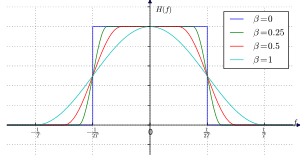
\includegraphics[width=5.8cm]{media/Hf-Raised-cosine_filter.png}    
                }
                \hfill
                \subfloat[$h_{(t)}$]{
                    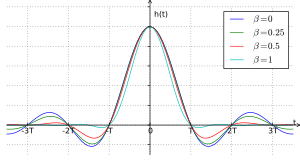
\includegraphics[width=5.8cm]{media/ht-Raised-cosine-impulse.png}    
                }
            \end{figure}

        }
        \item {
        }
    \end{enumerate}
    \subsection{Grandezze Energetiche}\label{Grandezze Fisiche}
        \textbf{Segnali tempo continui}
        \begin{itemize}
            \item {Potenza Istantanea
                \begin{align}
                    P_{x} & \triangleq |x_{(t)}|^2 \nonumber \\   
                    Se\ x_{(t)} \in &\ \mathbb{R} \rightarrow P_{x} \triangleq x_{(t)}^2 \nonumber
                \end{align}
            }
            \item {Energia
                \[
                    E_{x} \triangleq \int_{-\infty}^{\infty} P_{x}(t) \,dt = \int_{-\infty}^{\infty} |x_{(t)}|^2 \,dt    
                \]
                \begin{itemize}
                    \item Se $x_{(t)}$ ha $E_x < \infty \Rightarrow P_x = 0$
                    \item Se $x_{(t)}$ ha $P_x = k \neq 0 < \infty \Rightarrow E_x = \infty$
                \end{itemize}
                Parseval:\ref{Th. di Parseval}
                \[
                    E_{x} = \int_{-\infty}^{\infty}|x_{(t)}|^2 dt = \int_{-\infty}^{\infty}|X_{(f)}|^2 df =\int_{-\infty}^{\infty} S_{x(f)} df
                \]
            }
            \item {Potenza Media
                \[
                    P_{x} \triangleq \lim_{T\rightarrow\infty} \frac{E_{x_{T}}}{T} =\lim_{T\rightarrow\infty} \frac{1}{T} \int_{-\frac{T}{2}}^{\frac{T}{2}}  |x_{(t)}|^2 \,dt    
                \]  
            }
            \item {Valore Efficace
                \[    
                    x_{eff} \triangleq \sqrt{P_{x}}
                \]
            }
            \item {Valore Medio
                \[
                    x_{m} \triangleq \lim_{T\rightarrow\infty} \frac{1}{T} \int_{-\infty}^{\infty}  x_{(t)_T} \,dt = \lim_{T\rightarrow\infty} \frac{1}{T} \int_{-\frac{T}{2}}^{\frac{T}{2}}  x_{(t)} \,dt 
                \]
            }
        \end{itemize}
    \subsection{TSF}
        \[
            X_k =\frac{1}{T_0}\int_{-\frac{T_0}{2}}^{\frac{T_0}{2}} x_{(t)} e^{-j2\pi kf_0t} dt \hspace{1cm} x_{(t)} = \sum_{k = -\infty}^{\infty} X_{k} e^{j2\pi kf_0t} 
        \]
    \subsection{TCF}
        \[X_{(f)} = \int_{-\infty}^{\infty} x_{(t)} e^{-j2\pi ft} dt\hspace{1cm} x_{(t)} = \int_{-\infty}^{\infty} X_{(f)} e^{j2\pi ft} df\]
        \subsection{Proprietà}
            \begin{itemize}
                \item {Simmetria Hermitiana
                    \begin{align}
                        Ip&: x_{(t)}\ reale \nonumber \\
                        Th&: X_{(f)}\ hermitiana \nonumber \\ 
                        X_{(-f)} &= X_{(f)}^{*} \rightarrow
                            \begin{cases}
                                |X_{(f)}| = |X_{(-f)}| \hspace{0.3cm} & Simmetria\ Pari \\
                                \angle X_{(-f)} = -\angle X_{(f)}\hspace{0.3cm} & Simmetria\ Dispari
                            \end{cases} \nonumber
                    \end{align}
                }
                \item {Parità
                    \begin{align}
                        Ip&: x_{(t)}\ reale\ e\ pari  \nonumber \\
                        Th&: X_{(f)}\ reale\ e\ pari \nonumber  
                    \end{align}
                    }
                \item {Disparità
                    \begin{align}
                        Ip&: x_{(t)}\ reale\ e\ dispari  \nonumber \\
                        Th&: X_{(f)}\ immaginaria\ e\ dispari \nonumber 
                    \end{align}
                }
                \item{Linearità\\
                    $Ip: x_{(t)} = \alpha x_{1(t)} + \beta x_{2(t)}$\\        
                    $Th: X_{(f)} = \alpha X_{1(f)} + \beta X_{2(f)}$\\ 
                    Dimostrazione:
                    \begin{align}
                        X_{(f)} & = \int_{-\infty}^{\infty} (\alpha x_{1(t)} + \beta x_{2(t)}) e^{-j2\pi ft} dt \nonumber \\
                                & = \alpha \int_{-\infty}^{\infty} x_{1(t)} e^{-j2\pi ft} dt + \beta \int_{-\infty}^{\infty}  x_{2(t)} e^{-j2\pi ft} dt  \nonumber \\
                                & = \alpha X_{1(f)} + \beta X_{2(f)} \nonumber
                    \end{align}
    
                }
                \item{Dualità\\
                    $Ip: x_{(t)} \overunderset{TCF}{ATCF}{\leftrightharpoons} X_{(f)}$\\        
                    $Th: X_{(t)} \overunderset{TCF}{ATCF}{\leftrightharpoons} x_{(-f)}$ \\
                    Dimostrazione:
                    \begin{align}
                        X_{(f)} & = \int_{-\infty}^{\infty} x_{(t)} e^{-j2\pi ft} dt = Sost. \begin{cases}
                            t \rightarrow f\\
                            f \rightarrow t
                        \end{cases} \Rightarrow  X_{(t)} = \int_{-\infty}^{\infty} x_{(f)} e^{-j2\pi tf} df \nonumber \\
                                & =Sost.\ (f^\prime = -f) \Rightarrow  X_{(t)} = \int_{-\infty}^{\infty} x_{(-f^\prime)} e^{-j2\pi t(-f^\prime)} df^\prime\nonumber \\
                                & =\int_{-\infty}^{\infty} x_{(-f^\prime)} e^{j2\pi tf^\prime} df^\prime= ACTF[x_{(-f)}] = c.v.d.  \nonumber
                    \end{align}
                }
                \item{Ritardo\\
                    $Ip: \begin{cases}
                        x_{(t)} \overunderset{TCF}{ATCF}{\leftrightharpoons} X_{(f)} \nonumber \\
                        y_{(t)} = x_{(t-to)} \nonumber
                    \end{cases}$\\
                    $Th: Y_{(f)} \overunderset{TCF}{ATCF}{\leftrightharpoons} y_{(t)} = X_{(f)}e^{-j2\pi ft_0}$\\ 
                    Dimostrazione:
                    \begin{align}
                        Y_{(f)} & = \int_{-\infty}^{\infty} y_{(t)} e^{-j2\pi ft} dt = \int_{-\infty}^{\infty} x_{(t-t_0)} e^{-j2\pi tf} dt \nonumber \\
                                & =Sost.\ (t^\prime = t-t_0) \Rightarrow  Y_{(f)} = \int_{-\infty}^{\infty} x_{(t^\prime)} e^{-j2\pi f(t^\prime+t_0)} dt^\prime \nonumber \\
                                & =\int_{-\infty}^{\infty} x_{(t^\prime)} e^{-j2\pi ft^\prime}e^{-j2\pi ft_0} dt^\prime= X_{(f)}e^{-j2\pi ft_0}\ c.v.d.  \nonumber
                    \end{align}
                }
                \item{Derivazione\\
                    $Ip:\begin{cases}
                        x_{(t)}\overunderset{TCF}{ATCF}{\leftrightharpoons} X_{(f)}\\
                        y_{(t)}= \derivative{}{t} x_{(t)}        
                    \end{cases}$\\
                    $Th: Y_{(f)} = j2\pi f X_{(f)} $ \\
                    Dimostrazione:\\
                    \begin{align}
                        y_{(t)} &= \derivative{}{t} x_{(t)} = \derivative{}{t} ACTF[x_{(t)}] =\derivative{}{t} \int_{-\infty}^{\infty} X_{(f)}e^{j2\pi ft} df = \nonumber\\
                                &= \int_{-\infty}^{\infty} X_{(f)}\derivative{}{t}e^{j2\pi ft} df = \int_{-\infty}^{\infty} X_{(f)}j2\pi fe^{j2\pi ft} df \nonumber
                    \end{align}
                    Posso Scrivere $y_{(t)}$ come $ACTF[y_{(t)}] = \int_{-\infty}^{\infty} Y_{(f)}e^{j2\pi ft} df $, se quindi $Y_{(f)} = j2\pi f X_{(f)}$ l'ugaglianza è valida:
                    \[
                        y_{(t)} =\int_{-\infty}^{\infty} Y_{(f)}e^{j2\pi ft} df
                    \]
                    L'operazione di derivata nel dominio della frequenza si traduce in una semplice operazione algebrica, nel tempo avrei dovuto calcolare il 
                    rapporto incrementale. Per derivare un segnale posso quindi:
                    \begin{gather}
                        x_{(t)} \rightarrow TCF \rightarrow j2\pi fX_{(f)} \rightarrow ACTF \rightarrow y_{(t)}\nonumber
                    \end{gather}
                }
                \item{Integrazione\\
                    $Ip:\begin{cases}
                        x_{(t)} \overunderset{TCF}{ATCF}{\leftrightharpoons} X_{(f)}\ (1)\\
                        y_{(t)} = \int_{-\infty}^{t} x_{(\alpha)} d\alpha\ (2) \\
                        \int_{-\infty}^{\infty} x_{(t)} dt\ oppure\ \eval*{X_{(f)}}_{f=0} = 0 \ oppure\ y{(+\infty)} = 0\ (3) \\
                    \end{cases}$\\
                    $Th: Y_{(f)} =\frac{X_{(f)}}{j2\pi f}$ \\
                    Dimostrazione:\\
                    \begin{gather}
                        y_{(t)} = \int_{-\infty}^{t} x_{(\alpha)} d\alpha \Rightarrow {\color{purple}\derivative{}{t}} x_{(t)} = {\color{purple}\derivative{}{t}} y_{(t)} \overset{Th. \ref{Derivazione}}{\Rightarrow}  X_{(f)} = j2\pi f Y_{(f)} \nonumber\\
                                Y_{(f)} =\frac{X_{(f)}}{j2\pi f}\nonumber
                    \end{gather}
        
                    L'ipotesi 3 è conseguenza della divisione per $f$ e che devo mantenere l'uguaglianza $X_{(f)} = j2\pi f Y_{(f)}$, si nota come nella dimostrazione usando il Th della Derivazione (\ref{Derivazione})
                    quando $f=0$ la funzione nella frequenza deve essere $0,\ X_{(f)} = j2\pi f Y_{(f)} = 0$ 
                
                }
                \item{Integrazione Completo\\
                    $Ip:\begin{cases}
                        x_{(t)} \overunderset{TCF}{ATCF}{\leftrightharpoons} X_{(f)}\\
                        y_{(t)} = \int_{-\infty}^{t} x_{(\alpha)} d\alpha
                    \end{cases}$\\
                    $Th: Y_{(f)} =\frac{X_{(0)}}{2}\delta_{(f)} +\frac{X_{(f)}}{j2\pi f}$ \\
                    
                    Prende la denominazione di completo perché risolve il problema di mantenere l'uguaglianza $j2\pi fY_{(f)} = X_{(f)}$
                    
                }
                \item{Convoluzione\\
                    \[
                        z_{(t)} = x_{(t)} \otimes  y_{(t)} \triangleq \int_{-\infty}^{\infty} x_{(\tau)}y_{(t-\tau)} d\tau
                    \] 
                    $Ip:\begin{cases}
                        x_{(t)}\overunderset{TCF}{ATCF}{\leftrightharpoons} X_{(f)} \\
                        x_{(t)}\overunderset{TCF}{ATCF}{\leftrightharpoons} X_{(f)} \\
                        z_{(t)} = x_{(t)} \otimes  y_{(t)}   
                    \end{cases}$\\
                    $Th: Z_{(f)} = X_{(f)}Y_{(f)} $ \\
                    Dimostrazione:
                        \begin{align}
                            Z_{(f)} &= \int_{-\infty}^{\infty} z_{(t)} e^{-j2\pi ft} dt = \int_{-\infty_{t}}^{\infty}\int_{-\infty_{\tau}}^{\infty} x_{(\tau)}y_{(t-\tau)} e^{-j2\pi ft} dt\ d\tau \nonumber \\
                                    &= \int_{-\infty_{t}}^{\infty}x_{(\tau)}\int_{-\infty_{\tau}}^{\infty} y_{(t-\tau)}e^{-j2\pi ft}  dt\ d\tau \overset{Th. \ref{Ritardo}}{\Rightarrow} \int_{-\infty}^{\infty}Y_{(f)}x_{(\tau)}e^{-j2\pi f\tau} d\tau  \nonumber \\
                                    &= X_{(f)}Y_{(f)} \nonumber
                        \end{align}
                    Proprietà della convoluzione:
                    \begin{itemize}
                        \item {
                                Commutativa:
                                \[
                                    z_{(t)} = x_{(t)} \otimes  y_{(t)} = y_{(t)} \otimes  x_{(t)}  
                                \]
                                Dimostrazione:
                                \begin{align}
                                    z_{(t)} &= \int_{-\infty}^{\infty} x_{(\tau)}y_{(t-\tau)} d\tau \Rightarrow \tau=t-\tau^\prime\Rightarrow \int_{-\infty}^{\infty} x_{(t-\tau^\prime)}y_{(\tau^\prime)} d\tau^\prime \nonumber \\
                                            &= \int_{-\infty}^{\infty} y_{(\tau^\prime)}x_{(t-\tau^\prime)} d\tau^\prime = y_{(t)} \otimes  x_{(t)}\nonumber 
                                \end{align}
                            }
                        \item {
                                Associativa:
                                \[
                                    (x_{(t)} \otimes  y_{(t)}) \otimes z_{(t)}  =x_{(t)} \otimes  (y_{(t)} \otimes z_{(t)})   
                                \]
                            }
                        \item {
                                Distributiva:
                                \[
                                    x_{(t)} \otimes  (y_{(t)}+z_{(t)}) = x_{(t)}\otimes  y_{(t)} +x_{(t)}\otimes  z_{(t)}  
                                \]
                                Dimostrazione:
                                \begin{align}
                                    z_{(t)} &= \int_{-\infty}^{\infty} x_{(\tau)}(y_{(t-\tau)}+z_{(t-\tau)}) d\tau = \int_{-\infty}^{\infty}x_{(\tau)}y_{(t-\tau)} +x_{(\tau)}z_{(t-\tau)} d\tau \nonumber \\
                                            &= \int_{-\infty}^{\infty}x_{(\tau)}y_{(t-\tau)} d\tau +\int_{-\infty}^{\infty}x_{(\tau)}z_{(t-\tau)} d\tau = x_{(t)}\otimes  y_{(t)} +x_{(t)}\otimes  z_{(t)} \nonumber 
                                \end{align}
                            }
                    \end{itemize}
                }
            \end{itemize}
        \subsection{Relazione TCF-TSF Poisson}
            \[
                y_{(t)} \overset{TSF}{\rightleftharpoons}\overunderset{+\infty}{k = -\infty}{\sum} \frac{1}{T_0} X_{(kf_0)} e^{j2\pi kf_0t}    
            \]
        \subsection{Relazione TCF-TDF}
            la $TDF$ si ottiene periodicizzando la $TCF$ con periodo $\frac{1}{T}$:
            \[
                \overline{X}_{(f)} = \frac{1}{T} \sum_{n=-\infty}^{\infty} X_{(f-\frac{k}{T})} 
            \] 
    \subsection{Trasformate notevoli}
        \begin{itemize}
            \item {Gradino:\\
                \[
                    U_{(f)} = TCF[u_{(t)}] = \frac{1}{2}\delta_{(f)}+\frac{1}{2j\pi f}
                \]
            }
            \item {Delta di Dirac\\
                \begin{gather}
                    A\delta_{(t)} \overunderset{TCF}{ATCF}{\leftrightharpoons} A \nonumber \\
                    Per\ la\ dualita\ \ref{Dualita}: \nonumber \\
                    A \overunderset{TCF}{ATCF}{\leftrightharpoons} A\delta_{(-f)} = A\delta_{(f)}  \nonumber 
                \end{gather}
                Caso con ritardo:
                \begin{align}
                    A\delta_{(t-t_0)} &\overunderset{TCF}{ATCF}{\leftrightharpoons} Ae^{-j2\pi ft_0} \nonumber \\
                    Per\ la\ &dualita\ \ref{Dualita}: \nonumber \\
                    Ae^{-j2\pi f_0t} &\overunderset{TCF}{ATCF}{\leftrightharpoons} A\delta_{(-f-f_0)} =  A\delta_(f+f_0) \nonumber 
                \end{align}
            }
            \item {$cos$
                \[
                    \cos(2\pi f_0t) \overunderset{TCF}{ATCF}{\rightleftharpoons} \frac{\delta_{(f-f_0)}}{2} +\frac{\delta_{(f+f_0)}}{2}
                \]
            }
            \item {$sin$
                \[
                    \sin(2\pi f_0t) \overunderset{TCF}{ATCF}{\rightleftharpoons} \frac{\delta_{(f-f_0)}}{2j} -\frac{\delta_{(f+f_0)}}{2j}
                \]
            }
            \item{
                \[
                    A\hspace{0.1cm}rect\left(\frac{t}{T}\right) \overunderset{TCF}{ATCF}{\leftrightharpoons} AT sinc(fT)
                \]
            }
            \item {
                \begin{gather}
                    A\left(1-\left(\frac{|t|}{T}\right)\right)rect \left(\frac{t}{2T}\right) \rightleftharpoons ATsinc^2(fT)\nonumber\\
                    per\ la\ dualita \ref{Dualita}: \nonumber \\
                    ABsinc^2(Bt) \rightleftharpoons A\left(1-\left(\frac{|f|}{B}\right)\right)rect \left(\frac{f}{2B}\right) \nonumber
                \end{gather}                
            }
            \item {Funzione $sgn$\\
                \begin{align}
                    \frac{1}{t} &\overunderset{TSF}{ATSF}{\rightleftharpoons}  sgn(f) \nonumber \\
                    \text{Per la }&\text{Dualità \ref{Dualita}}\nonumber \\
                    sgn(t) &\overunderset{TSF}{ATSF}{\rightleftharpoons} \frac{1}{j\pi f} \nonumber
                \end{align}
            }
            \item{
                \[\sum_{n=-\infty}^{\infty}\delta_{(t-nT)} \overset{TDF}{\rightleftharpoons} \frac{1}{T} \sum_{k=-\infty}^{\infty} \delta_{(f-\frac{k}{T})}\nonumber\]
            }
        \end{itemize} 
    \subsection{TDF}
        \[
            \overline{X}_{(f)} = \sum_{n=-\infty}^{\infty} x_{[nT]}e^{-j2\pi fnT} \hspace{1cm} x_{[nT]} = \frac{1}{2\pi} \int_{2\pi} \overline{X}_{(f)}e^{j2\pi fnT} df
        \]
    \subsection{Modulazione in ampiezza}    
        \begin{itemize}
            \item {Con $cos$\\
                $Ip:\begin{cases}
                    y_{(t)}= x_{(t)}\cos(2\pi f_0t)\\        
                    x_{(t)}\overunderset{TCF}{ATCF}{\leftrightharpoons} X_{(f)}
                \end{cases}$\\
                \[ Y_{(f)} = \frac{1}{2} X_{(f-f_0)} + \frac{1}{2} X_{(f+f_0)}\]
            }
            \item {Con $sin$\\
                $Ip:\begin{cases}
                    y_{(t)}= x_{(t)}\sin(2\pi f_0t)\\        
                    x_{(t)}\overunderset{TCF}{ATCF}{\leftrightharpoons} X_{(f)}
                \end{cases}$\\
                \[Y_{(f)} = \frac{1}{2j} X_{(f-f_0)} - \frac{1}{2j} X_{(f+f_0)} \]
            }
            \item {Con $cos+\phi$\\
                $Ip: \begin{cases}
                    y_{(t)}= x_{(t)}\cos(2\pi f_0t + \phi)\\        
                    x_{(t)}\overunderset{TCF}{ATCF}{\leftrightharpoons} X_{(f)}
                    \end{cases}$\\
                \[Y_{(f)} = \frac{e^{j\phi}}{2} X_{(f-f_0)} + \frac{e^{-j\phi}}{2} X_{(f+f_0)} \]
            }
            \item {Con $complex$\\
                $Ip: \begin{cases}
                    y_{(t)}= x_{(t)}e^{j2\pi f_0t}\\        
                    x_{(t)}\overunderset{TCF}{ATCF}{\leftrightharpoons} X_{(f)}
                    \end{cases}$\\
                \[Y_{(f)} = X_{(f-f_0)} \]
            }
        \end{itemize}
    \subsection{Delta di Dirac}
        \[
            u_{(t)} = \int_{-\infty}^{\infty} \delta_{(t)} dt \rightarrow U_{(t)}
        \]
        \begin{itemize}
            \item {
                $\int_{-\infty}^{\infty} \delta_{(t)} dt = 1$
            }
            \item {
                Proprietà Campionatrice:\\
                $Ip:\ x_{(t)}\ continua\ in\ t_0$
                \[
                    \int_{-\infty}^{\infty}x_{(t)}\delta_{(t-t_0)} dt = x_{(t_0)}  
                \]
            }
            \item {
                Parità: $\delta_{(t)} = \delta_{(-t)}$
            }
            \item {
                $x_{(t)}\delta_{(t-t_0)} dt = x_{(t_0)}\delta_{(t-t_0)}$
            }
            \item {
                $x_{(t)} \otimes \delta_{(t)} = x_{(t)}$
            }
            \item {
                $x_{(t)} \otimes \delta_{(t-t_0)} = x_{(t-t_0)}$
            }
            \item {
                $U_{(f)} = TCF[u_{(t)}] = \frac{1}{2}\delta_{(f)}+\frac{1}{2j\pi f}$
            }
        \end{itemize}
    \subsection{Sistemi Monodimensionali}
        Il sistema applica la trasformazione $T[\ ]: y_{(t)} = T[x_{(t)}]$ in generale \\ $y_{(t)} = T[x_{(\alpha)},t]$. 
        Proprietà dei Sistemi Lineari Tempo Invarianti (LTI):
        \begin{itemize}
            \item {Linearità:
                \[
                    x_{(t)} = ax_{1(t)}+bx_{2(t)} \overset{T[\ ]}{\Rightarrow} y_{(t)} = aT[x_{1(t)}]+b T[x_{2(t)}]
                \]
                Oppure separando la variabile del tempo:
                \[
                    x_{(t)} = ax_{1(t)}+bx_{2(t)} \overset{T[\ ]}{\Rightarrow} y_{(t)} = aT[x_{1(\alpha)},t]+b T[x_{2(\alpha)},t]
                \]
                É il principio di linearità o sovrapposizione degli effetti visto a elettrotecnica.
            }
            \item {Stazionarietà:
                \[
                    y_{(t)} = T[x_{(t)}] \rightarrow y_{(t-t_0)} = T[x_{(t-t_0)}]  
                \]
            }
            \item {Causalità:
                \[
                    y_{(t)} = T[x_{(\alpha)},\alpha\leq t]
                \]
                L'uscita all'istante $t$ dipende dall'ingresso ad instanti precedenti o al più uguali a $t$, si basa su valori precedenti a 
                $t$ non può prevedere il futuro. Ne derivano 2 distinzioni di trasformazioni:
            }
            \item {Stabilità BIBO:
                Se il segnale $x_{(t)}$ ha ampiezza limitata $\rightarrow$ l'uscita ha ampiezza limitata:
                    \[
                        |x_{(t)}|\leq M \rightarrow |y_{(t)}|\leq K 
                    \]
            }
            \item {Invertibilità:
                \[
                    y_{(t)} = T[x_{(\alpha)},t] \overset{\text{Se} \exists}{\Rightarrow} x_{(t)} = T^{-1}[y_{(\alpha)},t]
                \]
            }
            \item {Memoria:
                Un sistema é:
                \begin{itemize}
                    \item {Senza memoria: se $y_{(t)} = T[x_{(\alpha)},\alpha=t]$}
                    \item {Con Memoria: $y_{(t)} =\int_{-\infty}^{t}x_{(\alpha)} d\alpha$ l'uscita all'istante $t$ dipende anche da valori dell'ingresso 
                          ad istanti diversi da $t$. Nota bene è l'integrale di convoluzione di $x_{(t)} \otimes u_{(t)}$ 
                    }
                \end{itemize}
            }
        \end{itemize}
        \subsubsection{Risposta impulsiva}
            $h_{(t)} \triangleq T[\delta_{(t)}]$\\
            $h_{(t)} \triangleq T[x_{(t)}] = x_{(t)}\ast h_{(t)} = \int_{-\infty}^{\infty}x_{(\alpha)}h_{(t-\alpha)}d\alpha$\\
            SLS causale se $h_{(t)} = h_{(t)}\ast u_{(t)}$ 
            SLS stabile se $\int_{-\infty}^{\infty}|h_{(t)}| dt < +\infty$ 
        \subsubsection{Risposta frequenza}
            l'uscita del sistema è quindi 
            \[
                Y_{(f)} = X_{(f)}\otimes H_{(f)}
            \]
            $H_{(f)}$ posso calcolarla in 3 modi:
            \begin{itemize}
                \item {
                    Utilizzando un impulso di Dirac e le sue proprietà, ma l'impulso di Dirac è difficile da realizzare. 
                }
                \item {
                    Calcolo $H_{(f)}$ mandando in ingresso un segnale del quale sia nota la sua risposta e calcolo il rapporto uscita/ingresso 
                    $H_{(f)} = \frac{Y_{(f)}}{X_{(f)}}$
                }
                \item {
                    Mandando in ingresso un esponenziale:
                    \[
                        y_{(t)} = x_{(t)}\otimes h_{(t)},\ x_{(t)} = e^{j2\pi f_0t}
                    \]
                    \begin{align}
                        y_{(t)} &= \int_{-\infty}^{\infty}x_{(t-\alpha)}h_{(t)}d\alpha = \int_{-\infty}^{\infty}h_{(\alpha)} e^{j2\pi f_0(t-\alpha)}d\alpha \nonumber \\
                                &= e^{j2\pi f_0t}\int_{-\infty}^{\infty}h_{(\alpha)} e^{j2\pi f_0\alpha}d\alpha = x_{(t)}H_{(f_0)} \nonumber 
                    \end{align}
                    \[
                        H_{(f_0)} = \frac{y_{(t)}}{x_{(t)}}
                    \]  
                    Posso calcolare la risposta in $f_0$, posso variare la frequenza e calcolare $H_{(f)} = \eval*{\frac{y_{(t)}}{x_{(t)}}}_{x_{(t)} = e^{j2\pi ft}}$
                }
            \end{itemize}

        \subsubsection{Sistemi in cascata}
            \[
                \text{Risposta Impulsiva}: h_{(t)} = h_{1(t)}\otimes h_{2(t)}
            \]
            \[
                \text{Risposta in Frequenza}: H_{(f)} = H_{1(f)} H_{2(f)}
            \]
        \subsubsection{Sistemi in parallelo}
            \[
                \text{Risposta Impulsiva}: h_{(t)} = h_{1(t)}+h_{2(t)}
            \]
            \[
                \text{Risposta in Frequenza}: H_{(f)} = H_{1(f)} + H_{2(f)}
            \]
    \subsection{Filtri}
        \begin{itemize}
            \item {LP
                \paragraph{Risposta in frequenza:}
                    $H_{LP(f)}\triangleq rect\left(\frac{f}{2B}\right)  $
                \paragraph{Risposta impulsiva:}
                    $h_{LP(t)}\triangleq 2Bsinc(2Bt)  $
            }
            \item {HP
                \paragraph{Risposta in frequenza:}
                   $ H_{HP(f)}\triangleq 1 - rect\left(\frac{f}{2B}\right)  $
                \paragraph{Risposta impulsiva:}
                    $h_{HP(t)}\triangleq \delta_{(t)} - 2Bsinc(2Bt)  $
            }
            \item {BP
                \paragraph{Risposta in frequenza:}
                  $  H_{BP(f)}\triangleq H_{LP(f+f_0)} +H_{LP(f-f_0)} =  rect\left(\frac{f-f_0}{2B}\right) + rect\left(\frac{f+f_0}{2B}\right)  $
                \paragraph{Risposta impulsiva:}
                    $h_{BP(t)}\triangleq 2Bsinc(2Bt) \cos(2\pi f_0t) = h_{LP(t)}\cos(2\pi f_0t)   $
            }
            \item {BS
                \paragraph{Risposta in frequenza:}
                  $  H_{BS(f)}\triangleq 1 -(H_{BP(f+f_0)} +H_{BP(f-f_0)}) = 1- \left[ rect\left(\frac{f-f_0}{2B}\right) + rect\left(\frac{f+f_0}{2B}\right)\right]  $
                \paragraph{Risposta impulsiva:}
                    $h_{BS(t)}\triangleq \delta_{(t)} - h_{BP(t)} = \delta_{(t)} - 2Bsinc(2Bt) \cos(2\pi f_0t)$
            }
        \end{itemize}
        \subsubsection{Filtro non distorcente}
            \begin{itemize}
                \item {Tempo: $H_{(f)} = k\delta_{(t-t_0)}$}
                \item {Frequenza: $H_{(f)} = ke^{-j2\pi ft_0}$}
            \end{itemize}
    \subsection{Teorema del campionamento}
        Consideriamo un segnale $x_{(t)}$ strettamente limitato in banda, cioè $X_{(f)} = 0 \forall |f|>B$, allora
        $x_{(t)}$ è completamente noto quando lo sono i valori
        \[
            x_{(nT)} \hspace{0.5cm} n\in\mathbb{Z},\ T\leq \frac{1}{T}  
        \]
        Le quantità $x_{(nT)}$ sono i campioni del segnale, mentre $T$ è il periodo di campionamento. La frequenza di
        campionamento limite F = 2B è la frequenza di Nyquist.

    \subsection{Teoria della probabilità}
        \begin{itemize}
            \item {P. Condizionata:\\
                Prendiamo in esempio un esperimento che implica due eventi $A$ e $B$: $P[A|B]$ sia la probabilità che un evento $A$ si verifichi
                dato il verificarsi dell'evento $B$, $P[A|B]$ è detta probabilità condizionata di $A$ dato $B$, assumendo $P[B]\neq 0$:
                \[
                    P[A|B] = \frac{P[A\cap B]}{P[B]}
                \]
            }
            \item {Regola di Bayes:\\
                Supponiamo che si possano ricavare facilmente le probabilità $P[A|B]$, $P[A]$ e $P[B]$ e vogliamo trovare la probabilità condizionata $P[B|A]$:
                \[
                    P[B|A] = \frac{P[A|B]P[B]}{P[A]}   
                \]
            }
            \item {Indipendenza:\\
                Supponiamo che l'occorrenza  di un evento $A$ non fornisca nessuna informazione sull'evento $B$, $P[B|A] = 0$. Dalla regola di Bayes abbiamo $P[A|B] = P[A]$,
                i due eventi sono indipendenti e occorre che:
                \[
                    P[A\cap B] = P[A]P[B]    
                \]
            }
            \item {Legge della probabilità totale:\\
                Supponiamo $\{ A_n = 1,\dots N\}$ è un insieme di eventi disgiunti:
                \[
                    P[B] = \sum_{n=1}^{N}P[B\cap A_n]    
                \]
            }
        \end{itemize}
    \subsection{Variabili aleatorie}
        \subsubsection{Funzione di distribuzione}
            Considera la variabile aleatoria $X$ e la probabilità dell'evento $X\leq x$, per convenzione si indica con $P[X\leq x]$,
            che può essere scritto come:
            \[
                F_{X(x)} \triangleq P[X\leq x]\ \forall x    
            \]
            La funzione $F_{X(x)}$ è chiamata la \emph{funzione distribuzione} della variabile $X$, si può notare che è funzione di $x$ non di 
            $X$.
        \subsubsection{Funzione di densità di probabilità}
            La variabile aleatoria $X$ è continua se la funzione distribuzione $F_{X(x)}$ è differenziabile:
            \[
                f_{X(x)} = \derivative{}{x}F_{X(x)}\ \forall x    
            \]
            $f_{X(x)}$ è detta \emph{funzione di densità di probabilità} (pdf).
        \subsubsection{Funzione Probabilità di massa - Probability Mass Function (pmf)}
            Consideriamo il caso di una variabile aleatoria discreta $X$, la quale può assumere un numero finito o infinito di valori. La funzione 
            distribuzione $F_{X(x)}$ si applica anche alle variabili discrete, ma non è differenziabile per come l'abbiamo definita. Definiamo 
            la funzione probabilità di massa $p_{X(x)}$:
            \[
                p_{X(x)} \triangleq P[X = x]    
            \]
            è la probabilità di un evento $X=x$, che consiste in tutti i possibili risultati di un esperimento i quali hanno un valore di 
            $X$ uguale a $x$.
        \subsubsection{Variabili multiple}
            Consideriamo due variabili aleatorie $X$ e $Y$:
            \begin{itemize}
                \item {
                    La funzione distribuzione $F_{X,Y (x,y)}$ è la probabilità che $X$ sia minore o uguale a un valore specifico $x$ e che $Y$
                    sia minore o uguale a un'altro valore specifico $y$:
                    \[
                        F_{X,Y (x,y)} = P[X\leq x,Y\leq y]    
                    \]
                }
                \item {
                    La funzione densità di probabilità $f_{X,Y (x,y)}$ contiene tutto quello che ci serve per fare una completa analisi della probabilità
                    di più variabili aleatorie:
                    \[
                        f_{X,Y (x,y)} = \frac{d^2 F_{X,Y (x,y)}}{dxdy}     
                    \]

                }
            \end{itemize}
        \subsubsection{Funzione probabilità condizionata}
            Supponendo che $X$ e $Y$ siano due variabili aleatorie continue con $f_{X,Y (x,y)}$, la funzione densità di probabilità condizionata di $Y$ con $X=x$,
            è definita da:
            \[
                f_{Y (y|x)} = \frac{f_{X,Y (x,y)}}{f_{X(x)}}     
            \]
            Supponendo che le due variabili siano indipendenti: allora $f_{Y (y|x)}$ si riduce alla densità marginale $f_{Y (y)}$ e la funzione densità di
            probabilità diventa $f_{X (x)}f_{Y (y)}$, se così fosse le due variabili si dicono \emph{statisticamente indipendenti}.
        \subsubsection{Somma di variabili aleatorie indipendenti}
            Consideriamo due variabili aleatorie $X$ e $Y$ statisticamente indipendenti e continue con funzioni di densità di probabilità $f_{X (x)}$ e $f_{Y (y)}$ si 
            definisce $Z = X+Y$ la cui $pdf$ $f_{Z (z)}$ é:
            \[
                f_{Z (z)} = \int_{-\infty}^{\infty}f_{X (x)}f_{Y (z-x)} dx =  f_{X (x)} \otimes f_{Y (y)}
            \]
            La somma di due variabili aleatorie indipendenti e continue è la convoluzione delle funzioni di densità di probabilità.
        \subsubsection{Valore medio - Expectation}
            L'expectation o il valore medio di una variabile aleatoria continua $X$ è formalmente definito da:
            \begin{itemize}
                \item {Caso Continuo:
                    \[
                        \mu_X = \mathbb{E}[X] = \int_{-\infty}^{\infty} xf_{X(x)}dx
                    \]
                }
                \item {Caso Discreto:
                    \[
                        \mathbb{E}[X] = \sum_{x}xp_{X(x)}
                    \]
                }
            \end{itemize}
            è la media pesata delle variabili aleatorie, può anche essere un valore che non gli appartiene.
        \subsubsection{Varianza}
            La varianza $\sigma^2_x$ di una variabile aleatoria $X$ è definita:
            \[
                var[X] = \mathbb{E}[(X-\mu_X)^2] = \int_{-\infty}^{\infty} (X-\mu_X)^2f_{X(x)}dx
            \]  
            \begin{align}
                var[X] &= \sigma^2_x \overset{\ref{linearita expectation}}{=} \mathbb{E}[X^2-2\mu_XX+\mu_X^2] = \mathbb{E}[X^2]-2\mu_X\mathbb{E}[X]+\mu_X^2 \nonumber \\
                        &= \mathbb{E}[X^2]-\mu_X^2 \nonumber 
            \end{align}\index{Valore quadratico medio}
            $\mathbb{E}[X] = \int_{-\infty}^{\infty} xf_{X(x)}dx$ mentre $\mathbb{E}[X^2] = \int_{-\infty}^{\infty} x^2f_{X(x)}dx$, l'expectation è il peso che diamo alla funzione $f_{X(x)}$.  
            Misura la "randomicità" di una variabile aleatoria, meno è randomica più sono vicino al mio valor medio.
            \[
                P[|X-\mu_X|\geq \mathcal{E}]\leq \frac{\sigma^2_X}{\mathcal{E}^2}
            \]
        \subsubsection{Deviazione standard}
            $\sigma_X = \sqrt[2]{\sigma^2_X}$
        \subsubsection{Covarianza}  
            Siano $X$ e $Y$ due variabili aleatorie, si definisce covarianza:
            \begin{gather}
                cov[XY] = \mathbb{E}[(X-\mathbb{E}[X])(Y-\mathbb{E}[Y])]\nonumber\\
                = \mathbb{E}[XY]-\mu_X\mu_Y\nonumber
            \end{gather}
        \subsubsection{Coefficiente di correlazione}
            Il \emph{coefficiente di correlazione} di $X$ e $Y$ é:
            \[
                \rho_{(X,Y)} = \frac{cov[XY]}{\sigma_X\sigma_Y}
            \]
            misura la somiglianza tra $X$ e $Y$. Le due variabili si dicono:
            \begin{itemize}
                \item {
                    Incorrelate: se la $cov[XY] =0$, ciò non implica l'indipendenza delle variabili.
                }
                \item {
                    Ortogonali: se $\mathbb{E}[XY] = 0$
                }
            \end{itemize}
    \subsection{Distribuzione Gaussiana}
        Una variabile aleatoria $X$ è detta Gaussiana se la funzione distribuzione di probabilità ,$pdf$, ha la forma:
        \[
            f_{X(x)} = \frac{1}{\sqrt{2\pi}\sigma_X}e^{\left[\displaystyle -\frac{(x-\mu_X)^2}{2\sigma^2_X}\right]}  
        \]
        \paragraph{Proprietà:}\label{proprietà distr gaussiana}
        \begin{itemize}
            \item {Definita unicamente dal valore medio di $X$ e la varianza $\mathcal{N}(\mu_X,\sigma_X^2)$.}
            \item {\begin{sloppypar}
                La proprietà di Gaussianità è preservata dalle trasformazioni lineari. ${X \sim \mathcal{N}(\mu_X,\sigma_X^2): Y = \alpha X+\beta}$, calcoliamo come variano 
                valor medio e varianza:
            \end{sloppypar}
                \begin{itemize}
                    \item {Valor medio:
                        \[
                            \mathbb{E}[Y] = \mu_Y = \mathbb{E}[\alpha X+\beta]  \overset{\ref{linearita expectation}}{=} \alpha \mathbb{E}[X] + \beta
                        \]
                    }
                    \item {Varianza:
                        \begin{align}
                            \sigma_Y^2  &= \mathbb{E}[Y^2] -\mathbb{E}[Y]^2 =\mathbb{E}[(\alpha X + \beta)^2] -(\alpha \mathbb{E}[X] + \beta)^2 \nonumber \\
                                        &= \mathbb{E}[\alpha^2 X^2 + \beta^2 +2\alpha\beta X] -(\alpha^2 \mathbb{E}[X]^2 + \beta^2 +2\alpha\beta\mathbb{E}[X])\nonumber \\
                                        &= \alpha^2 \mathbb{E}[X^2] + \beta^2 +2\alpha\beta \mathbb{E}[X] -\alpha^2 \mathbb{E}[X]^2 - \beta^2 -2\alpha\beta\mathbb{E}[X]\nonumber \\
                                        &= \alpha^2 \mathbb{E}[X^2] -\alpha^2 \mathbb{E}[X]^2 = \alpha^2 (\mathbb{E}[X^2] -\mathbb{E}[X]^2)\nonumber \\
                                        &= \alpha^2 (\mathbb{E}[X^2] -\mu_X^2)=\alpha^2 \sigma_X^2\nonumber
                        \end{align}                         
                        la costante $\beta$ non influisce la varianza.  
                    }
                \end{itemize}}
            \item {La somma $Z = X+Y$ di variabili aleatorie Gaussiane indipendenti è anche essa una variabile aleatoria
                Gaussiana, con:
                    \begin{itemize}
                        \item {$\mathbb{E}[Z] = \mathbb{E}[X] +\mathbb{E}[Y] $}
                        \item {$var[Z] = var[X] +var[Y] $}
                    \end{itemize}}
        \end{itemize}
        \subsubsection{Gaussiana Standard}
            Si dice forma Gaussiana Standard se: $\mathbb{E}[X] = 0$ e $var[X] = 1$, $\mathcal{N}(0,1)$:
            \begin{gather}
                f_{X(x)} = \frac{1}{\sqrt{2\pi}} e^{\displaystyle\left(-\frac{x^2}{2}\right)}\nonumber \\
                F_{X(x)} =P[X\leq x] = \int_{-\infty}^{\infty}f_{X(x)} =\frac{1}{\sqrt{2\pi}} \int_{-\infty}^{x}e^{\displaystyle\left(-\frac{t^2}{2}dt\right)}\nonumber 
            \end{gather}
        \subsubsection{Funzione $Q$}
            \[
                Q_{(x)} = 1-F_{X(x)} = P[X\geq x]  
            \]
            formalmente è cosi definita:
            \[
                Q_{(x)} = 1-F_{X(x)} = 1 - \frac{1}{\sqrt{2\pi}} \int_{-\infty}^{x}e^{\left(-\frac{t^2}{2}dt\right)} = \frac{1}{\sqrt{2\pi}} \int_{x}^{\infty}e^{\left(-\frac{t^2}{2}dt\right)}  
            \]
            è l'area sottesa dalla funzione di distribuzione Gaussiana da $x$ all'infinito
            \paragraph{Proprietà:}
            \begin{itemize}
                \item {$Q_{(x)} = 1-Q_{(-x)}$
                }
                \item {$Q_{(\infty)} = 0$}
                \item {$Q_{(-\infty)} = 1$}
                \item {$Q_{(0)} = \frac{1}{2}$}
            \end{itemize}
            \subsubsection{Errore sul simbolo}
                \[
                    Q_{\displaystyle\left(\frac{\lambda -\mu_Y}{\sigma_Y}\right)} = P_r[n>\lambda + \mu_Y]
                \]
        \subsubsection{Th. del valore centrale}
            Siano $X_1,\dots,X_n$ una sequenza di variabili aleatorie indipendenti e identicamente distribuite con valore medio $\mu$ e varianza $\sigma$:
            \[
                Y_n = \frac{1}{\sigma\sqrt{n}}\left(\sum_{i=1}^{n}X_i-n\mu\right)    
            \]
            al tendere di $n$ all'infinito, $Y_n$ converge alla variabile aleatoria Gaussiana standard:
            \[
                F_{Y(y)} =P[Y\leq y] = \frac{1}{\sqrt{2\pi}} \int_{-\infty}^{y}e^{\left(-\frac{x^2}{2}\right)}dx    
            \]
    \subsection{Processi stocastici}
        \subsubsection{Valore medio}
            \[
                \mu_{X(t)} = \mathbb{E}[X_{(t)}] = \int_{-\infty}^{\infty}xf_{X_{(t)}(t)}dt
            \]
        \subsubsection{Autocorrelazione}
            \[
                R_{XX(t_1,t_2)} = \mathbb{E}[X_{t_1}X_{t_2}] = \int_{-\infty}^{\infty}\int_{-\infty}^{\infty} x_1x_2f_{X_{(t_1)},X_{(t_2)}(x_1,x_2)}dx_1dx_2
            \]  
            Proprietà:
            \begin{itemize}
                \item {$R_{X(0)}=P_x = \underset{Potenza}{\underbrace{\mathbb{E}[|X|^2]}} = \int_{-\infty}^{\infty} x^2f_{X_{(t)}(t)}dx$}
            \end{itemize}
        \subsubsection{Densità spettrale di potenza}
            \[
                S_{XX(f)} = \lim_{T\rightarrow+\infty}\frac{1}{T}|X_{(f)}|^2 \overset{TCF[R_{XX}]}{=} \int_{-\infty}^{\infty} R_{XX(\tau)} e^{-j2\pi f\tau}d\tau
            \]
            Proprietà:
            \begin{itemize}
                \item {$P_x = \int_{-\infty}^{\infty} S_{XX(f)} df$}
                \item {$S_{Y} = \frac{1}{T} S_{XX(f)} |H_{(f)}|^2$}
            \end{itemize}
    \subsection{Sistemi SSL}
        Un processo stocastico $X_{(t)}$ si dice Stazionario in Senso Lato (SSL) se:
        \begin{itemize}
            \item {Il valore medio del processo $X_{(t)}$ è costante $\forall t$:
                \[
                    \mu_{X(t)} = \mathbb{E}[X_{(t)}] \overset{SSL}{\Rightarrow} \mu_{X}    
                \]
            }
            \item {La funzione di autocorrelazione del processo $X_{(t)}$ dipende solamente dalla differenza tra la differenza 
                tra due tempi qualsiasi al quale il processo è campionato:
                \[
                    R_{XX(t_1,t_2)} = \mathbb{E}[X_{(t_1)}X_{(t_2)}] \overset{SSL}{\Rightarrow} R_{X(t_1-t_2)} = R_{X(\tau)}      
                \]
                Se il processo dipende solo da $\tau$ posso farne la $TCF$ e analizzarne la densità spettrale. 
                }
        \end{itemize}
        \subsubsection{Uscita del sistema SSL}
            \begin{itemize}
                \item {Valor medio: $\mu_Y= \mu_X H_{(0)}$}
                \item {Autocorrelazione: $R_{YY(t_1,t_2)} = R_{X(\tau)} \otimes h_{(t_1)}\otimes h_{(t_2)}$
                }
                \item {$S_{Y} = \frac{1}{T} S_{XX(f)} |H_{(f)}|^2$}
                \item {$P_{Y} = \frac{1}{T} \int_{-\infty}^{\infty} S_{XX(f)} |H_{(f)}|^2$}
            \end{itemize}
    \subsection{Processo Gaussiano}
        Un processo $Y_{(t)}$ è detto processo Gaussiano se la variabile aleatoria $Y$ è una variabile aleatoria a distribuzione Gaussiana:
        \[
            f_{Y(y)} = \frac{1}{\sqrt{2\pi}\sigma}e^{\left(\displaystyle-\frac{(y-\mu)^2}{2\sigma^2}\right)}    
        \]
    \subsection{Modello sistema di comunicazione}
        Trasmissione:
        \begin{figure}[H]
            \centering
                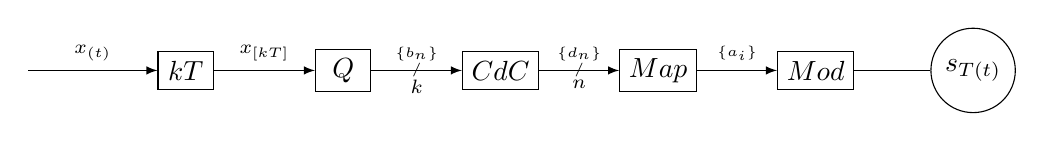
\begin{tikzpicture}[
                        node distance=2cm,
                        >=latex
                    ]
                    % Blocks
                    \node [coordinate] (input) {};
                    \node [rectangle, draw,minimum height=1em, minimum width=2em,right of=input] (AD) {$kT$};
                    \node [rectangle, draw,minimum height=1em, minimum width=2em,right of=AD] (Q) {$Q$};
                    \node [rectangle, draw,minimum height=1em, minimum width=2em,right of=Q] (CS) {$CdC$};
                    \node [rectangle, draw,minimum height=1em, minimum width=2em,right of=CS] (CC) {$Map$};
                    \node [rectangle, draw,minimum height=1em, minimum width=2em,right of=CC] (TX) {$Mod$};
                    \node [circle,draw,right of=TX] (TXant) {$s_{T(t)}$};
                
                    % Connections
                    \draw [->] (input) --node[above]{\scriptsize$x_{(t)}$} (AD);
                    \draw [->] (AD) --node[above]{\scriptsize$x_{[kT]}$} (Q);
                    \draw [->] (Q) --node[above]{\tiny$\{b_n\}$}node[midway]{\tiny$/$} node[below]{\scriptsize$k$} (CS);
                    \draw [->] (CS) --node[above]{\tiny$\{d_n\}$}node[midway]{\tiny$/$} node[below]{\scriptsize$n$} (CC);
                    \draw [->] (CC) --node[above]{\tiny$\{a_i\}$} (TX);
                    \draw [-] (TX) -- (TXant);
                \end{tikzpicture}    
            \caption{Esempio sistema di trasmettitore}
        \end{figure}
        Al livello di codificatore ho:\\
        $R_b = \frac{1}{T_b}$ è il Bit Rate a cui i bit sono generati in ingresso mentre, $R_d = \frac{1}{T_d}$ è il Bit Rate di uscita. Volendo trovare la relazione tra ingresso e uscita:
        \[
            kT_b = nT_d \Rightarrow \frac{R_b}{R_d} = \frac{k}{n}     
        \] 
        al mappatore:\\
        il periodo $T$ tra due \emph{simboli} adiacenti viene detto "Intervallo di Segnalazione". Se $M=2^q$ allora:
        \[
            T = qT_d =T_d log_{2}(M)  
        \]
        la velocità di trasmissione dei simboli $f_s = \frac{1}{T}$ è legata al rate $R_d$ da:
        \[
            f_s = \frac{R_d}{Q} = \frac{R_d}{log_{2}(M)} 
        \]
        al modulatore:\\
        la banda impiegata sarà:
        \[
            B_T \simeq \frac{1}{T}  
        \]
        volendolo esprimere in relazione ai vari bit rate:
        \[
            B_T = \frac{1}{T} \overset{T = qT_d}{=} \frac{1}{qT_d} = \frac{1}{T_d log_2(M)} = \frac{R_b}{\frac{n}{k} log_2(M)}     
        \]
    \subsection{PAM}
        \begin{itemize}
            \item {Modulatore:$s_{T(t)} = \sum_{i}a_ig_{T(t-iT)}$}
            \item {Densità spettrale di potenza:
                \begin{gather}
                    S_{s(f)} = \frac{1}{T} S_{a(f)}\left|G_{T(f)}\right|^2 \nonumber \\
                    S_{a(f)} = \sum_{m} R_{a(m)}e^{-j2\pi fmT} \nonumber
                \end{gather}  
            }
            \item {Potenza:
                \begin{gather}
                    P_s = \frac{1}{T}\int_{-\infty}^{\infty}S_{a(f)} \left|G_{T(f)}\right|^2 df \nonumber\\
                    S_{a(f)} = \sigma_a^2 + \frac{\eta_a^2 }{T}\sum_{k} \delta_{(f-\frac{k}{T})} \nonumber \\
                    S_{s(f)} \overset{\eta_a^2 = 0}{=} \frac{\sigma_a^2}{T} \left|G_{T(f)}\right|^2 = \frac{\mathbb{E}[a_i^2]}{T} \left|G_{T(f)}\right|^2 = \frac{R_{a(0)}}{T} \left|G_{T(f)}\right|^2 \nonumber
                \end{gather}
                e la potenza:
                \[
                    P_s  = \frac{\sigma_a^2}{T} E_{g_T} = \frac{\mathbb{E}[a_i^2]}{T} E_{g_T} = \frac{R_{a(0)}}{T} E_{g_T}
                \]
            }
            
            \item {Caso IID:
                \begin{itemize}
                    \item {Densità spettrale di potenza:
                        \[
                            S_{s(f)} = \frac{M^2-1}{3T}\left|G_{T(f)}\right|^2
                        \]
                    }
                    \item {Potenza:
                        \[
                            P_s = \frac{M^2-1}{3T}E_{g_T}
                        \]
                    }
                    \item {Energia media per simbolo: dato che l'energia è calcolata in un $\Delta t$ posso ricavare l'energia del simbolo moltiplicando la potenza per $T$
                        \[
                            E_S = P_sT = \frac{M^2-1}{3}E_{g_T}
                        \]
                    }
                    \item {Energia media per bit: dato che l'energia è calcolata in un $\Delta t$ posso ricavare l'energia del bit da trasmettere
                    moltiplicando la potenza per $T_d$
                        \[
                            E_d = P_sT_d = \frac{M^2-1}{3log_2(M)}E_{g_T}
                        \]
                    }
                \end{itemize}
            }
            \item {Ricevitore:\\
                Componente Ricevuta:$x_{[kT]} = \sum_{i}a_ig_{[(n-i)T]}+n_{[k]}$
                isolando il termine $m=0$
                \[
                    x_{[kT]} = a_Kg_{(0)} + \sum_{m\neq 0}a_{k-m}g_{[mT]}+n_{[k]}    
                \]
            }
            \item {Annullamento ISI:\\ 
                $g_{[mT]} = 
                \begin{cases}
                    1   &per \ m=0\nonumber \\
                    0   &per \ m\neq 0\nonumber
                \end{cases}$
                in frequenza\\
                $
                \begin{cases}
                    g_{(0)} & m=0\nonumber \\
                    0 &\nonumber
                \end{cases}  \Rightarrow \overline{G_{(f)}} = g_{(0)} 
                $
                con banda massima pari a $B=\frac{1}{2T}$
            }
        \end{itemize}
    \subsection{Filtro adattato}
        \[
            H_{(f)} = TCF[p_{(t_0-t)}] = P^*_{(f)}e^{-j2\pi ft_0}    
        \]
        applicandolo ai filtri in trasmissione e ricezione con annullamento di ISI e massimizzazione dell'SNR
        \[
            g_{R(t)} = g_{T(-t)} \Rightarrow G_{R(f)} = G_{T(f)}^\ast
        \]
        \[
            G_{(f)} = G_{T(f)} G_{R(f)} = G_{RCR(f)} 
        \]
        il filtro deve quindi essere
        \[
            G_{T(f)} = \sqrt{G_{RCR(f)}} = G_{R(f)}    
        \] 
    \subsection{Criterio MAP}
        Voglio massimizzare la probabilità di 
        corretta ricezione 
        \[
            P_r[a_k = a^{(i)}|x_{[k]}] = \frac{f_x[x_{[k]}|a_k = a^{(i)}]P_r[a_k = a^{(i)}]}{f_x[x_{[k]}]}    
        \]
        se i simboli non sono equiprobabili
        \[
            \Gamma_{(a^{(i)},x_{[k]})} = \left[x_{[k]}-a^{(i)}\right]^2-2\sigma^2ln(P_i)
        \]
        In caso di simboli equiprobabili diventa il criterio a massima verosimiglianza
        \[
            \left(x_{[k]}-a^{(i)}\right)^2<\left(x_{[k]}-a^{(\ell)}\right)^2  
        \]
    \subsection{Efficienza Spettrale}
        \[
            \eta_{sp} = \frac{R_d}{B_T} [\frac{bit}{Hz}]    
        \]
        dove $R_d=\frac{log_2(M)}{T}$ è il bit-rate
    \subsection{Codifica di GRAY}
        \[
            BER \simeq \frac{2(M-1)}{Mlog_2(M)}Q_{\displaystyle \left(\sqrt{\frac{6log_2(M)}{M^2-1}}\frac{E_d}{N_0}\right)}    
        \] 
    \subsection{QAM}
        \begin{itemize}
            \item {Trasmettitore:
                l'inviluppo complesso del segnale trasmesso è 
                \[
                    \tilde{s}_{(t)} = I_{(t)} +j Q_{(t)}      
                \]
                e il segnale trasmesso
                \[
                    s_{T(t)} = \mathbb{R}e\{\tilde{s}_{(t)}e^{j\omega_0t}\}
                \]
                Densità spettrale: $S_{s(f)} = \frac{1}{4}\left[S_{\tilde{s}{(f-f_0)}}+ S_{\tilde{s}{(-f-f_0)}}\right]$
                \[
                    S_{\tilde{s}{(f)}} = \frac{1}{T} f_{c(f)}\left|G_{T(f)}\right|^2    
                \]
                dove 
                \[
                    f_{c(f)} = \sum_{m}R_{c(m)}e^{-j2\pi fmT}
                \]
                è la densità spettrale di potenza dei simboli complessi $\{c_i\}$. La potenza di $s_{T(t)}$ è quindi esprimibile come
                \[
                    P_s=\frac{1}{2T} \int_{-\infty}^{\infty} f_{c(f)} \left|G_{T(f)}\right|^2 df
                \]
                Poiché $g_{T(t)}$ è un impulso tipicamente a radice di coseno rialzato, la banda di $\tilde{s}_{T(t)}$ è 
                \[
                    B_{\tilde{s}}=\frac{1+\alpha}{2T}    
                \]
                la banda del segnale trasmesso $s_{T(t)}$ 
                \[
                    B_{T}=2B_{\tilde{s}} =\frac{1+\alpha}{T}
                \]
                e l'efficenza spettrale del sistema risulta 
                \[
                    \eta_{sp} = \frac{R_d}{B_T} = \frac{log_2(M)}{1+\alpha} 
                \]
            }
            \item {Ricevitore:

            }
        \end{itemize}
            
    \subsection{Modulazione ASK}
        la densità spettrale di potenza dell'impulso complesso è 
        \[
            S_{\tilde{s}(f)} = \frac{M^2-1}{3T}\left|G_{T(f)}\right|^2
        \]
        e l'energia media per simbolo trasmesso è 
        \begin{align}
            E_s &= \frac{1}{2}T\int_{-\infty}^{\infty}S_{\tilde{s}(f)}df\nonumber \\
                &= \frac{M^2-1}{6}E_{g_T}\nonumber
        \end{align}
        essendo $E_{g_T}$ l'energia di $g_{T(t)}$. Qualora $g_{T(t)}$ sia un impulso a radice di coseno rialzato, l'efficenza spettrale
        del sistema ASK è 
        \[
            \eta_{sp} = \frac{log_2(M)}{1+\alpha}    
        \]
    \subsection{Modulazione QAM}
        la densità spettrale di potenza dell'inviluppo complesso è 
        \[
            S_{\tilde{s}(f)} = \frac{C_2}{T}\left|G_{T(f)}\right|^2    
        \]
        dove 
        \[
            C_2 = \mathbb{E}[\left|c_i\right|^2] = \frac{2}{3}(M-1)    
        \]
        è la potenza media dei simboli trasmessi. Possiamo calcolare l'energia media per simbolo trasmesso
        \[
            E_s = \frac{1}{2}T\int_{-\infty}^{\infty}S_{\tilde{s}(f)} df = \frac{M-1}{3}E_{g_T}
        \]
        con $E_{g_T}$ energia di $g_{T(t)}$. Qualora $g_{T(t)}$ sia un impulso a radice di coseno rialzato, l'efficenza spettrale del 
        sistema QAM diventa 
        \[
            \eta_{sp} = \frac{log_2(M)}{1+\alpha}  
        \]
        In presenza di codifica di GRAY, la BER è espressa approssimativamente da 
        \[
            BER \simeq \frac{4(\sqrt{M}-1)}{\sqrt{M}log_2(M)}Q_{\displaystyle \left(\sqrt{\frac{3log_2(M)}{M-1}\frac{E_d}{N_0}}\right)}  
        \]
    \subsection{Codice ISBN}
        \begin{itemize}
            \item {Codifica:
                \begin{enumerate}
                    \item {
                        Si calcola la grandezza $z = mod(S,11)$ con
                        \[
                            S = \sum_{j=1}^{9} (11-j)x_{(j)}
                        \]
                    }
                    \item {
                        La cifra di controllo di parità è il complemento a 11 di $z$:
                        \[
                            x_{(10)} = mod(11-z,11)  
                        \]
                        E solo per la cifra di controllo di parità se $x_{(10)} = 10$ si sostituisce con 
                        $x_{(10)} = X$
                    }
                \end{enumerate} 
            }
            \item {Decodifica:
                \begin{enumerate}
                    \item {
                        Moltiplica ogni cifra per il peso della posizione della stessa cifra e calcola $mod(S^\prime,11)$ con
                        \[
                            S^\prime = \sum_{j=1}^{10} (11-j)y_{(j)}
                        \]
                    }
                    \item {
                        Assumendo che non ci siano errori su $x_{(10)} = |11-z|_{11}$, si ha:
                        \begin{align}
                            mod(S^\prime,11) &= mod \left( \sum_{j=1}^{9} (11-j)y_{(j)} + mod(11-z,11),11\right) \nonumber \\
                                            &= mod \left( \sum_{j=1}^{9} (11-j)y_{(j)} + \left(11-\sum_{j=1}^{9} (11-j)x_{(j)}\right),11\right)\nonumber \\
                                            &= mod \left(\sum_{j=1}^{9} (11-j)(y_{(j)}-x_{(j)}),11\right)
                        \end{align}
                    }
                \end{enumerate}
                Se non ci sono errori si ha $y=x$ e quindi il $mod(S^\prime,11) = 0$
                \paragraph{Rivelazione degli errori:} Il codice è in grado di rivelare tutti i singoli errori:
                sia $e_{(k)}$ l'errore in posizione $k$,$y_{(k)} = x_{(k)}+ e_{(k)}$:
                \[
                    mod(S^\prime,11) = mod((y_{(k)}-x_{(k)})(11-k),11)+mod(e_{(k)}(11-k),11) \neq 0
                \]
            }
        \end{itemize}
    \subsection{Distanza di Hamming}
        La distanza di Hamming tra due vettori, o stringhe, $d(x_1,x_2)$ di $n$ elementi è il numero di posizioni in cui le due parole
        sono diverse tra loro
    \subsection{Peso di Hamming}
        Il peso di Hamming,$w(x)$, di una stringa i lunghezza $n$ è la sua distanza di Hamming dal vettore di $n$ zeri,
        $x_0\in \mathcal{V}_n$ é:
        \[
            w(x_0) = d(x_0,0_n)
        \]
    \subsection{Distanza minima}    
        La distanza minima di un codice $\mathcal{C}$ è la minima distanza di Hamming calcolata fra tutte le possibili parole che appartengono a $\mathcal{C}$.
        \[
            d_{min} (\mathcal{C})= \underset{x_1,x_2 \in \mathcal{C}}{min}d(x_1,x_2)  
        \]
        \paragraph{Teorema:} La distanza minima del codice a blocco $\mathcal{C}(k,n)$ si può calcolare come il 
            peso di Hamming minimo tra tutte le parole di codice:
            \begin{align}
                d_{min}(\mathcal{C}) &= \underset{x_i,x_j\in\mathcal{C}}{\min} d_H(x_i,x_j) = \underset{x_i,x_j\in\mathcal{C}}{\min} d_H(x_i+x_j,x_j+x_j)\nonumber \\
                                        &= \underset{x_i,x_j\in\mathcal{C}}{\min} d_H(x_i+x_j,0_{1,n}) \overset{[x_i+x_j\in\mathcal{C}]}{\Rightarrow} \underset{x_i\in\mathcal{C}}{\min}\ w(x_i)\nonumber
            \end{align}
    \subsection{Codici a blocco}
        Sia $u = [u_1, \dots, u_k]$ una generica parola di $k$ cifre binarie. Il codice a blocco lineare $\mathcal{C}(k,n)\subset \mathcal{V}_n$ è l'insieme delle
        $2^k$ parole $x = [x_1, \dots, x_n]$ di $n$ cifre binarie ottenute con la trasformazione lineare:
        \[
            x = uG  
        \]
        \subsubsection{Forma sistematica}
            Quando il codice è in forma sistematica la matrice generatrice del codice ha la seguente forma:
            \begin{gather}
                G = [I_k,P]\nonumber \\
                G\in k\times n,\ I\in k\times k,\ P\in k\times (n-k)\nonumber
            \end{gather}
            dove la matrice $P$ è la matrice di parità
        \subsubsection{Matrice di controllo di parità}
            La matrice $H$ è la matrice di controllo di parità del codice. Per costruzione $\forall x \in \mathcal{C}$ vale:
            \begin{gather}
                    xH^T = uGH^T = 0 \nonumber \\
                    H\in (n-k) \times n\nonumber 
            \end{gather}
            La matrice $H$ non è unica, ma se il codice è sistematico posso ricavarla in un'altra forma:
            \begin{gather}
                H = [P^T,I_{n-k}] = 0 \nonumber \\
                H\in (n-k) \times n,\ I\in (n-k)\times (n-k),\ P^T\in (n-k) \times k \nonumber
            \end{gather}
            Se fosse $\neq 0$ ciò che è stato ricevuto non è una parola di codice.
        \subsubsection{Error detection}
            Sia $x$ la parola di codice trasmessa e $y=x+e$ la corrispondente sequenza di $n$ bit ricevuta. supponiamo che il canale 
            introduca un numero di errori:$w(e) > 0$, si dice:
            \begin{itemize}
                \item {
                    Errore Rivelabile\index{Errore Rivelabile}: se $y$ non è una parola di codice, $y\notin\mathcal{C}(k,n) $
                }
                \item {
                    Errore Non Rivelabile\index{Errore Non Rivelabile}: se $y$ è una parola di codice ma non quella trasmessa, $w(e) \geq d_{min}$ 
                }
            \end{itemize}
        \subsubsection{Decodifica a massima verosimiglianza}
            \paragraph{Strategia}
                $\hat{x}$ che, tra tutte le $2^k$ possibili parole di codice $x$, massimizza la probabilità condizionata 
                $P(y|x)$:
                \[
                    \hat{x} = \arg \underset{x\in\mathcal{C}}{\max}\ P(y|x)
                \]
                Poiché gli eventi di errore sono indipendenti da bit a bit, posso riscrivere la probabilità condizionata come il prodotto delle probabilità condizionate
                ottenute per ciascun bit trasmesso:
                \[
                    P(y|x) = \prod_{\ell=1}^{n} P(y_\ell|x_\ell)
                \]
                La probabilità $P(y|x)$ si calcola:
                \[
                    P(y|x) = p^{d_H(x,y)}(1-p)^{n-d_H(x,y)} =(1-p)^{n}\left(\frac{p}{1-p}\right)^{d_H(x,y)} 
                \]
                Mi interessa scegliere un $x$ che massimizza $\left(\frac{p}{1-p}\right)^{d_H(x,y)}$, è un valore $<1$:
                \begin{itemize}
                    \item {
                        Se ho la $d_H(x,y)$ piccola ho la probabilità minore di errore.
                    }
                    \item {
                        Se ho la $d_H(x,y)$ alta ho la probabilità di errore alta.
                    }
                \end{itemize}
            \paragraph{Decisione}
                La parola di codice decisa $\hat{x}$ è quella che minimizza la distanza dalla parola $y$ ricevuta:
                \[
                    \hat{x} = \arg \underset{x\in\mathcal{C}}{\max}\ P(y|x) = \arg \underset{x\in\mathcal{C}}{\min}\ d_H(y,x)
                \]
                Scelgo $x$ tale che mi dia la minima distanza
                \subparagraph{Ricevitore ML ottimo:}\index{Ricevitore ML ottimo} Il ricevitore ML ottimo è il ricevitore a distanza minima, il ricevitore
                che associa alla sequenza di $n$ bit ricevuta $y$, la parola di codice $x$ che minimizza la $d_H(y,x)$.
                \subparagraph{Ricevitore ML error correction:}\index{Ricevitore ML error correction} Il ricevitore ML è in grado di correggere con successo tutti quegli errori
                $e$ per cui la parola ricevuta $y = x+e$ è comunque più vicina alla parola trasmessa $x$ che a qualsiasi altra parola del codice.
                
                Per ogni vettore $v\in\mathcal{V}_n$ e un raggio $r$ esiste una "sfera" di raggio $r$ i cui elementi sono tutti quei vettori in $\mathcal{V}_n$ che hanno
                distanza di Hamming da $v$ minore o uguale a $r$

            \paragraph{Capacità di correggere errori (Error Correction):}
                \subparagraph{Teorema:}\begin{sloppypar}
                Un codice lineare a blocco può correggere fino a ${t_{max} = \left\lfloor \frac{d_{min}-1}{2} \right\rfloor}$ errori: $2t_{max}+1 \leq d_{min} \leq 2t_{max}+2$.
                \end{sloppypar}
    \subsection{Codici di Hamming}
        I codici di Hamming $\mathcal{C}_H(m)$ sono definiti a partire da un parametro: $m \geq 2$
        \[
            n = 2^m-1,\ k = 2^m-m-1 = n-m
        \]
        \subparagraph{Matrice di controllo di parità:} per definizione la matrice $H \in (n-k)\times n$, ma per i codici di Hamming la matrice $H$ ha dimensione:
        $H \in m\times (2^m-1)$.

        \subparagraph{Matrice di parità:} Per un codice di Hamming sistematico la matrice di parità $P\in k \times m$ viene costruita così che le colonne di $H = [P^T,I_{n-k}]$
        siano tutte le possibili $2^m-1$ combinazioni di $m$ bit (esclusa la $n-upla$ di tutti 0)
        \subsubsection{Decodifica codici a blocco}
            Dato il vettore ricevuto:
            \[
                y = x+e
            \]
            Il decisore ottimo selezione la parola di codice $\hat{x}$:
            \[
                \hat{x} = \arg \underset{x\in\mathcal{C}}{\max}\ P(y|x) = \arg \underset{x\in\mathcal{C}}{\min}\ d_H(y,x)   
            \]
            Invece di stimare $\hat{x}$ si stima il vettore $\hat{e}$ più probabile
            \begin{align}
                \hat{e} &= \arg \underset{e}{\max}\ P(e|y+e\in\mathcal{C}) = \arg \underset{e|y+e\in\mathcal{C}}{\max}\ p^{w(e)}(1-p)^{n-w(e)} \nonumber \\
                        &= \arg \underset{e|y+e\in\mathcal{C}}{\max}\ \left(\frac{1-p}{p}\right)^{-w(e)} = \arg \underset{e|y+e\in\mathcal{C}}{\min}\ w(e)  \nonumber 
            \end{align}
            La decodifica sceglie tra tutti i possibili vettori errore $e$ tali che $y+e\in\mathcal{C}$ quello che ha il peso di Hamming minimo, cioè il minimo numero di 
            errori (Massima Verosimiglianza). Una volta stimato $\hat{e}$:
            \[
                \hat{x} = y-\hat{e} = y+\hat{e} = x+(\hat{e}+e)=
                \begin{cases}
                    x &se\ \hat{e} = e\nonumber\\    
                    x_1\neq x &se\ \hat{e} \neq e\nonumber    
                \end{cases}     
            \]
        \subsubsection{Coset}
            Sia $\mathcal{C}(k,n)$ un codice a blocco e sia $v\in \mathcal{V}_n$ un vettore di $n$ cifre binarie, si definisce $coset$ di
            $\mathcal{C}(k,n)$ individuato da $v$ l'insieme:
            \[
                C_v = C+v=\{ x+v: x\in\mathcal{C} \}
            \]
            \paragraph{Proprietà dei coset}
            \begin{enumerate}
                \item {Qualsiasi vettore in $\mathcal{V}_n$ appartiene a un coset di $\mathcal{C}(k,n)$}
                \item {Ciascun coset contiene $2^k$ elementi}
                \item {Due coset o sono coincidenti o hanno intersezione nulla}
                \item {Ci sono $2^{n-k}$ coset distinti}
                \item {Se $v_1$ e $v_2$ appartengono allo stesso coset, $v_1 + v_2 \in \mathcal{C}(k,n)$ è una parola di codice}
            \end{enumerate}
            \paragraph{Algoritmo di decodifica}
            \begin{enumerate}
                \item Avendo ricevuto il vettore $y$ si trova un coset di appartenenza $\mathcal{C}_y$.
                \item {Si identifica il coset leader, la parola di peso minimo del coset $\mathcal{C}_y$, che è anche la parola di peso minimo del 
                coset di $\mathcal{C}_e$.}
                \item Il coset leader è la stima del vettore di errore $\hat{e}$
            \end{enumerate}
        \subsubsection{Decodifica mediante sindrome}
            Si definisce sindrome di $y$ il vettore $s$ ottenuto dal prodotto di $y$ con la matrice di controllo di parità:
            \[
                s = yH^T = (x+e)H^T = xH^T+eH^T = eH^T    
            \]
            \paragraph{Procedura di decodifica:}
                \begin{enumerate}
                    \item {Calcola la sindrome $s = yH^T$}
                    \item {Associa la sindrome al coset leader corrispondente $s\rightarrow e_{CL}(s)$}
                    \item {Corregge l'errore sommando il coset leader alla $n-upla\ y$}
                \end{enumerate}
                La parola $\hat{x}$ è una parola di codice:
                \[
                    \hat{x}H^T= (y+e_{CL}(s))H^T = s+s =0   
                \]
                e per costruzione la parola di codice $\hat{x}$ minimizza la distanza di Hamming da $y$
    \subsection{Codici ciclici}
        \paragraph{Shift Ciclico:}
            \begin{sloppypar}
                Dato il vettore ${v = [v_0,\dots,v_{n-1}]\in \mathcal{V} = G(2)^n}$ indichiamo con $v^{(i)}$ il vettore ottenuto da $v$ applicando uno 
                \emph{shift ciclico} di $i$ posizioni a destra:
                \[
                    v^{(i)} = [v_{n-i},v_{n-i+1}, \dots, v_{n-1},v_0,v_1,\dots, v_{n-i-1}]    
                \]     
            \end{sloppypar}
            Un codice lineare $\mathcal{C}(k,n)$ si definisce \emph{ciclico} se data una generica parola di codice $x\in \mathcal{C}(k,n)$ ogni suo
            shift ciclico $x^{(i)}\in \mathcal{C}(k,n)$. Sono codici a correzione d'errore che hanno proprietà algebriche che rendono sia la rivelazione che la correzione
            di errore efficienti.
        \subsubsection{Rappresentazione codici ciclici}
            A ciascun vettore $v = [v_0,\dots,v_{n-1}]\in \mathcal{V}$ è possibile associare un polinomio definito in $GF(2)$:
            \[
                v_{(D)} = v_0 + v_1 D+\dots+ v_{n-1}D^{n-1}    
            \]
            \paragraph{Proprietà:} Uno \emph{shift ciclico} di $i$ posizioni del vettore $v$ è equivalente a moltiplicare
            il polinomio $v_{(D)}$ per $D^i$ modulo $(D^n-1)$:
            \[
                v^{(i)} \rightleftharpoons \mod\{D^iv_{(D)},(D^n-1)\}    
            \]
        \subsubsection{Polinomio generatore}
            Il polinomio generatore di un codice ciclico $\mathcal{C}(k,n)$ è il polinomio
            \[
                g_{(D)} = 1+g_1D+ \dots + D^r    
            \]
            non nullo e di grado minimo in $\mathcal{C}(k,n)$.
        \subsubsection{Matrice generatrice di un codice ciclico}
            Dato il codice ciclico $\mathcal{C}(k,n)$ con polinomio generatore $g_{(D)}$ dal momento che l'insieme dei polinomi
            \[
                \{g_{(D)},Dg_{(D)},\dots,D^{k-1}g_{(D)}\}  
            \]
            costituisce una base per il codice, la matrice generatrice del codice è 
            \[
                G = 
                \begin{bmatrix}
                g_0 & g_1 & \dots & g_{n-k} & 0 & \dots & 0\\ 
                0 & g_0 & g_1 & \dots & g_{n-k} & \dots & 0\\ 
                \vdots &  &  &  &  &  & \vdots\\ 
                0 & \dots & 0 & g_{0} & \dots & g_{n-k-1} & g_{n-k}
                \end{bmatrix}
            \]
            considerato che $g_0 = 1$ le righe possono essere sommate tra loro per ottenere la matrice generatrice del codice 
            equivalente in forma sistematica $G = [I_k,P]$.
        \subsubsection{Matrice controllo parità di un codice ciclico}
            Dato il codice ciclico $\mathcal{C}(k,n)$ con polinomio generatore $g_{(D)}$ esiste sempre un polinomio 
            $h_{(D)} = h_0+h_1D+\dots+h_{(k)}D^k$ tale che 
            \[
                h_{(D)} = \frac{(D^n-1)}{g_{(D)}} \Rightarrow g_{(D)}h_{(D)} = D^n-1    
            \]
            Abbiamo un set di $n-k$ equazioni del tipo 
            \[
                v_m =  \sum_{j=0}^{n-1}x_{(j)}h_{(m-j)} = 0\ m=k,k+1,\dots,n-1  
            \]
            le equazioni possono essere riassunte nella forma matriciale
            \[
                xH^T=0_{n-k}  
            \]
            dove la matrice $H$ di dimensioni $(n-k)\times n$ è la matrice controllo di parità del codice ciclico $\mathcal{C}(k,n)$ 
            \[
                H = 
                \begin{bmatrix}
                h_k & h_{k-1} & \dots & h_{0} & 0 & \dots & 0\\ 
                0 & h_k & h_{k-1} & \dots & h_{0} & \dots & 0\\ 
                \vdots &  &  &  &  &  & \vdots\\ 
                0 & \dots & 0 & h_{k}& h_{k-1} & \dots  & h_0
                \end{bmatrix}
            \]
            il calcolo della sindrome può essere effettuato mediante:
            \[
                s = yH^T    
            \]
        \subsubsection{Metodo per il calcolo della sindrome}
            La sindrome associata alla matrice di controllo di parità sistematica si può calcolare
            usando un metodo alternativo. Al ricevitore si ha 
            \[
                y=x+e\Rightarrow y_{(D)} = x_{(D)}+e_{(D)}
            \]
            la sindrome può essere calcolata come il resto della divisione tra polinomi
            \[
                \frac{y_{(D)}}{g_{(D)}}\Rightarrow y_{(D)} = a_{(D)}g_{(D)} + s_{(D)} 
            \]
            \paragraph{Esempio decodifica di codici ciclici}
                Sia $x = [0110100]$ una parola del codice ciclico $\mathcal{C}(4,7)$ con polinomio generatore 
                $g_{(D)} = 1+D+D^3$. Sia $e = [0100000]$ l'errore introdotto dal canale. Il vettore ricevuto è 
                \[
                    y= x+e = [0010100]\rightleftharpoons y_{(D)} = D^2+D^4 
                \]
                da cui calcoliamo la sindrome 
                \[
                    s_{(D)} = mod\{y_{(D)},g_{(D)}\}=D
                \]
                ho quindi 
                \[
                    w_{(s_{(D)})} = 1\Rightarrow s_{(D)} =e_{(D)} = \hat{e} = [0100000]  
                \]
            \paragraph{Teorema:} Dato il codice ciclico $\mathcal{C}(k,n)$ sia $s_{(D)}$ la sindrome del vettore ricevuto
                $y$ allora la sindrome $s_{1(D)}$ della parola $y^{(1)}$ ottenuta dallo shift ciclico di $y$ di una posizione 
                si calcola:
                \[
                    s_{1(D)} = mod\left\{y^{(1)}_{(D)},g_{(D)}\right\} = Ds_{(D)}-s_{n-k-1}g_{(D)}    
                \]
                \paragraph{Esempio decodifica a sindrome di codici ciclici}
                Sia $x=[0110100]$ una parola del codice ciclico $\mathcal{C}(4,7)$ con polinomio generatore $g_{(D)} = 1 + D + D^3$
                ed $e=[0000010]$ l'errore introdotto dal canale. Il vettore ricevuto è 
                \[
                    y= x+e = [0110110]\rightleftharpoons y_{(D)} = D+D^2+D^4+D^5 
                \]
                da cui calcoliamo la sindrome 
                \[
                    s_{(D)} = mod\{y_{(D)},g_{(D)}\}=D^2+D+1
                \]
                Lo shift ciclico di $y$:
                \[
                    y^{(1)} = [001011] \rightleftharpoons y^{(1)}_{(D)} = D^2+D^3+D^5+D^6   
                \]
                \begin{align}
                    s_{1(D)} &= mod\left\{y^{(1)}_{(D)},g_{(D)}\right\}= D^2+1  \nonumber \\
                             &= D(D^2+D+1)-D^3+D+1 \nonumber
                \end{align}
                Lo shift ciclico di $y^{(1)}$:
                \[
                    y^{(2)} = [100101] \rightleftharpoons y^{(2)}_{(D)} = 1+D^3+D^4+D^6   
                \]
                \begin{align}
                    s_{2(D)} &= mod\left\{y^{(2)}_{(D)},g_{(D)}\right\}= 1 = D^2+1  \nonumber \\
                             &= D(D^2+D+1)-D^3+D+1 \nonumber
                \end{align}
    \subsection{Codici convoluzionali}
        Ad ogni tempo di bit il codificatore combina i bit
        all'interno di una finestra mobile di lunghezza $L$, chiamata \emph{constraint length} del codice, per generare gli $n$ 
        bit in uscita. Il processo di codifica può essere interpretato come una convoluzione in $GF(2)$ ed il codificatore di
        un codice convoluzionale $(n,k,L)$ si può rappresentare come $n$ filtri lineari in $GF(2)$ in parallelo.
        \subsubsection{Codificatore codice convoluzionale}
            Un codificatore convoluzionale è costituito da uno shift register e da sommatori: 
            \begin{itemize}
                \item {
                    \begin{sloppypar}
                        Ad ogni periodo di clock (definito dall'intero $i$) nel codificatore entrano $k$ (tipicamente $1$) cifre binarie 
                        rappresentate dal vettore ${u^{i} = [u^{i}_1,u^{i}_2,\dots,u^{i}_k]}$ ed escono $n$ bit raccolti nel vettore di uscita
                        ${x^{i} = [x^{i}_1,x^{i}_2,\dots,x^{i}_n]}$
                    \end{sloppypar}
                }
                \item {
                    All'interno del codificatore $u^{(i)}$ è combinato con i precedenti $L-1$ vettori di ingresso $u^{(i-1)},u^{(i-2)},\dots,u^{(i-L+1)}$
                    per formare l'uscita $x^{(i)}$
                }
            \end{itemize}
        \subsubsection{Generatore di un codice convoluzionale}
            I generatori definiscono completamente un codice convoluzionale, così come la matrice generatrice o il polinomio generatore definiscono
            definiscono i codici a blocco e i codici ciclici. Per i codici convoluzionali 
            \begin{itemize}
                \item {
                    A ciascuna delle $n$ uscite corrisponde generatore e a ciascun generatore corrisponde un sommatore in $GF(2)$.
                }
                \item {
                    Ciascun generatore ha $kL$ elementi uno per ciascun ingresso che contribuisce all'uscita del codificatore.
                }
                \item {
                    Quando un elemento è $1$ significa che il corrispondente ingresso è connesso al sommatore altrimenti se è $0$
                    non c'è connessione.
                }
            \end{itemize}
            I vettori generatori rappresentano la risposta impulsiva degli $n$ filtri lineari in $GF(2)$. Assumendo che $k=1$ il 
            generatore per il bit $m-esimo$ è $g_m = [g^{(0)}_m,g^{(1)}_m,\dots,g^{(L-1)}_m]$ e l'$m-esimo$ bit di uscita $x^{(i)}_m$ 
            si ottiene con 
            \[
                x_m^{(i)} = \sum_{\ell = 0}^{L-1} g_m^{(\ell)}u^{(i-\ell)}  
            \]
        \subsubsection{Rappresentazione come macchina a stati}
            Ad ogni istante di segnalazione l'uscita dal codificatore convoluzionale dipende 
            dall'ingresso attuale e dalla memoria. Le ultime $k(L-1)$ celle dello shift register memorizzano la 
            storia passata del codificatore che è riassunta nel vettore di stato 
            \[
                \sigma = \left(u^{(i-1)},u^{(i-2),\dots, u^{(i-L+1)}}\right)  
            \]
            Il codificatore può presentarsi come una macchina a stati finiti la cui evoluzione nel tempo
            è descritta da equazioni di stato 
            \begin{gather}
                x^{(i)} = \delta\left(u^{(i)},\sigma^{(i)}\right)\nonumber \\
                \sigma^{(i+1)} = \lambda\left(u^{(i)},\sigma^{(i)}\right)\nonumber 
            \end{gather}
            Il numero di stati complessivo è $2^{k(L-1)}$ con celle di memoria pari a $k(L-1)$.
        \subsubsection{Distanza colonna}
            Sia dato un codice convoluzionale $\mathcal{C}(n,k,L)$. Consideriamo $\mathcal{X}_\mathcal{C}(\ell,\sigma)$, l'insieme
            di tutte le possibili sequenze che originano dallo stato $\sigma$ e hanno lunghezza pari a $\ell n$, ottenute cioè dopo 
            $\ell$ passi sul traliccio. La \emph{distanza colonna} del codice $\mathcal{C}$ al passo $\ell$ è la minima distanza di Hamming
            fra due sequenze $x$ e $x^\prime$ in $\mathcal{X}_\mathcal{C}(\ell,\sigma)$ che siano differenti nei primi $n$ bit, in corrispondenza
            quindi della prima parola di uscita del codificatore 
            \[
                d_{c(\ell)} = \underset{\substack{x,x^\prime \in \mathcal{X}_\mathcal{C}(\ell,\sigma) \\ x^{(1)}\neq x^{\prime(1)} }}{min} d(x,x^\prime)  
            \]
        \subsubsection{Distanza libera}
            La distanza libera di un codice convoluzionale $\mathcal{C},d_{free}$ è il limite della distanza colonna per $\ell$ che tende 
            all'infinito
            \[
                d_{free} = \lim_{x\rightarrow \infty} d_{c(\ell)}  
            \]
            In pratica la distanza libera coincide con la distanza colonna quando i due percorsi sul traliccio a massima distanza confluiscono.
            La distanza libera, come la $d_{min}$ nei codici a blocco, è una misura della bontà del codice: tanto maggiore è la distanza libera 
            tanto più è difficile confondere due sequenze che originano dallo stesso stato.
        \subsubsection{Decodifica a massima verosimiglianza}
            fra tutte le $2^{kN}$ possibili sequenze di tentativo $\tilde{x}$, massimizza la probabilità 
            condizionata $P[y|\tilde{x}]$
            \[
                \hat{x} = arg\ \underset{\tilde{x}}{max}P[y|\tilde{x}]   
            \]
            la probabilità condizionata $P\left[y^{(\ell)}|\tilde{x}^{(\ell)}\right]$ si ottiene a partire dal calcolo della distanza di Hamming 
            $\lambda^{(\ell)}_{\tilde{x}} = d_H(y^{(\ell)},\tilde{x}^{(\ell)})$, infatti per ogni bit diverso tra le due parole di assume che ci sia stato errore e quindi 
            \[
                P\left[y^{(\ell)}|\tilde{x}^{(\ell)}\right] = p^{\lambda^{(\ell)}_{\tilde{x}}}(1-p)^{n-\lambda^{(\ell)}_{\tilde{x}}} = (1-p)^n\left(\frac{p}{1-p}\right)^{\lambda^{(\ell)}_{\tilde{x}}}
            \]
            Poiché la funzione logaritmo è crescente la sequenza di tentativi che massimizza $P[y|\tilde{x}]$ che massimizza anche $log\left(\lambda^{(\ell)}_{\tilde{x}}\right)$.
            Sostituendo la funzione \ref{eventi indipendenti} in quella appena calcolata e prendendone il logaritmo
            \[
                log\left(P\left[y^{(\ell)}|\tilde{x}^{(\ell)}\right]\right) =nNlog \left((1-p)^n\right) + log\left(\frac{p}{1-p}\right)\sum_{\ell=1}^{N}\lambda^{(\ell)}_{\tilde{x}}
            \]
            trascurando i termini ininfluenti e considerando che è lecito assumere $log\left(\frac{p}{1-p}\right)<0$ si ottiene la regola di decisione 
            \[
                \hat{x} = arg\ \underset{\tilde{x}}{max}P[y|\tilde{x}] = arg\ \underset{\tilde{x}}{min}\sum_{\ell=1}^{N}\lambda^{(\ell)}_{\tilde{x}}
            \]
            La strategia a massima verosimiglianza consiste nello scegliere la sequenza $\hat{x}$ che minimizza la distanza di Hamming dalla sequenza 
            ricevuta 
            \[
                d_H(y,\hat{x}) = \sum_{\ell=1}^{N}\lambda^{(\ell)}_{\tilde{x}}
            \]
    \subsection{Algoritmo di Viterbi}
        \begin{itemize}
            \item {Metrica di Ramo:$\sigma_j\rightarrow\sigma_k$ al passo $\ell$, a distanza di Hamming
                $\lambda^{(\ell)}= d_H(y^{(\ell)},\tilde{x}_{\sigma_j\rightarrow\sigma_k})$. La metrica è 
                calcolata come distanza tra la sequenza ricevuta al passo $\ell$ e l'uscita corrispondente
                alla transizione sul traliccio dallo stato $\sigma_j$e lo stato $\sigma_k$.
            }
            \item {Metrica Cumulata: al passo $f$ allo stato $\sigma_k$, la grandezza $\wedge_{x(\sigma_k)}^{(f)}$ ottenuta 
                sommando tutte le $f$ metriche di ramo calcolate su gli $f$ rami sul traliccio di un percorso $x$ che si fermi allo stato 
                $\sigma_k$ al passo $f$.
            }
        \end{itemize}
        L'algoritmo di Viterbi si basa sulla seguente intuizione:
        \begin{itemize}
            \item {Supponiamo che due diversi percorsi $x_1$ e $x_2$ confluiscano al passo $f$ nello stesso nodo $\sigma_k$
                sul traliccio e siano $\wedge_{x_1 (\sigma_k)}^{(f)}<\wedge_{x_2 (\sigma_k)}^{(f)}$ le metriche cumulate dei due
                percorsi calcolate al passo $f$.
            }
            \item {Supponiamo che al passo successivo $f+1$, i percorsi $x_1$ e $x_2$ seguano lo stesso
                ramo sul traliccio, ad esempio $\sigma_k\rightarrow\sigma_q$, in questo caso la metrica di ramo è la stessa per i due 
                percorsi $\lambda^{(f+1)}_{(\sigma_k,\sigma_q)}$. 
            }
            \item {Per le nuove metriche sarà ancora $\wedge_{x_1 (\sigma_q)}^{(f+1)}<\wedge_{x_2 (\sigma_q)}^{(f+1)}$
                infatti si ha 
                \begin{align}
                    \wedge_{x_1 (\sigma_q)}^{(f+1)} &= \wedge_{x_1 (\sigma_k)}^{(f)}+\lambda^{(f+1)}_{(\sigma_k,\sigma_q)} < \wedge_{x_2 (\sigma_k)}^{(f)}+\lambda^{(f+1)}_{(\sigma_k,\sigma_q)} \nonumber\\
                                                    &= \wedge_{x_2 (\sigma_q)}^{(f+1)}\nonumber
                \end{align}
            }
        \end{itemize}
        Generalizzando questa intuizione possiamo dire che:
        \begin{enumerate}
            \item {In un traliccio arrivato alla sua piena espansione ad ogni nuovo istante di segnalazione arrivano $2^k$ percorsi a ciascun nodo.}
            \item {I valori delle metriche di ramo in uscita da un nodo sono uguali per tutti i percorsi che arrivano a quel nodo.}
            \item {A parità di percorso futuro, il percorso in ingresso al nodo con la metrica cumulata minore continuerà ad avere metrica cumulata più bassa di tutti gli altri}
            \item {Ai fini della minimizzazione della metrica cumulata complessiva ad ogni nodo si possono scartare i $2^{k-1}$ percorsi con la metrica cumulata 
                più alta e conservare quello con la metrica cumulata minima
            }
            \item {l'unico percorso rimasto viene definito sopravvissuto}
        \end{enumerate}
    \subsection{Calcolo di errore sui bit}
        \subsubsection{Errore sul bit per una BPSK}
            $P_w(e)$ può essere limitato inferiormente dalla probabilità dell'evento più probabile: aver commesso $t+1$
            errori
            \[
                P_w(e) \simeq \binom{n}{t+1}p^{t+1}(1-p)^{n-(t+1)}
            \]
            mentre la $P_w(e)$ si riesce a calcolare con precisione, nel caso del calcolo della probabilità di errore 
            su bit codificato si deve per forza ricorrere ad approssimazioni. Il numero di bit errati in $\hat{x}$ dopo la 
            decodifica dipende dal vettore di errore $e$ e da come agisce la decodifica a sindrome, che in presenza di un numero 
            di errori maggiore di $t$ aggiunge altri errori a quelli introdotti dal canale. La decodifica a sindrome restituisce
            sempre una parola di codice, quindi ogni volta che al ricevitore c'è un errore nella decodifica i bit errati sono almeno
            $d_{min}$ negli $n$ trasmessi. in questo caso la $P_b(e)$ si approssima a
            \[
                P_b(e) \simeq\frac{d_{min}}{n}P_w(e)\simeq\frac{d_{min}}{n}\binom{n}{t+1}p^{t+1}(1-p)^{n-(t+1)}  
            \] 
            \paragraph{Senza codifica}
                \[
                    p_b^{(BPSK)}(e) = Q_{\displaystyle\left(\sqrt{\frac{2E_b}{N_0}}\right)}  
                \]
            \paragraph{Con codifica}
                nel caso codificato bisogna considerare che la probabilità di errore $p$ dipende dal valore di SNR dei bit codificati
                \[
                    \frac{E_{b,c}}{N_0} = \frac{k}{n} \frac{E_b}{N_0}    
                \]
                \[
                    p = Q_{\displaystyle\left(\sqrt{\frac{2E_{b,c}}{N_0}}\right)} = Q_{\displaystyle\left(\sqrt{2\frac{k}{n}\frac{E_{b,c}}{N_0}}\right)} 
                \]
        \subsubsection{Errore sul bit codici convoluzionali}
            La bontà di un codice convoluzionale dipende dalla sua $d_{free}$. La $d_{free}$ dipende
            dai codici generatori, dal rate $R= \frac{k}{n}$ e dalla constraint length $L$. Tipicamente i 
            codici convoluzionali hanno $k=1$ per limitare la complessità di codificatore e decodificatore. 
            Fissato $R$ e $L$ i generatori ottimi sono quelli che massimizzano la $d_{free}$ e possono essere trovati 
            tramite una ricerca esaustiva fra tutte le possibili $\left(2^L\right)^n = 2^{nL}$ combinazioni.
            \paragraph{Puncturing}
                la tecnica chiamata \emph{Puncturing} permette di costruire con codici con rate maggiori partendo da un codice
                a rate $R=\frac{1}{n}$. Il puncturing consiste nel cancellare alcuni bit all'uscita del codificatore.
                I bit vengono cancellati secondo un pattern preciso, espresso da una \emph{puncturing table}, condiviso
                con il ricevitore.
                \[
                    R^\prime = \frac{1}{n} \frac{nM}{P}=\frac{M}{P}  
                \]
            \paragraph{Errore sul bit}
                Ad alti rapporti segnale/rumore si trova la seguente approssimazione: BPSK codificata con 
                decodifica hard
                \[
                    P_e^{(b)} \simeq Q_{\displaystyle \left(\sqrt{2\frac{E_b}{N_0}\frac{R^\prime}{2}}\right)}  
                \] 
    \subsection{Varie}\label{Varie}
        \begin{itemize}
            \item {
                Calcolo della TCF su MATLAB:\\
                $X_{(f)} = \int_{-\infty}^{\infty} x_{(t)} e^{-j2\pi ft } dt$

                MATLAB calcola un'approssimazione dell'integrale della TCF con un periodo $T$:
                \begin{figure}[H]
                    \centering
                    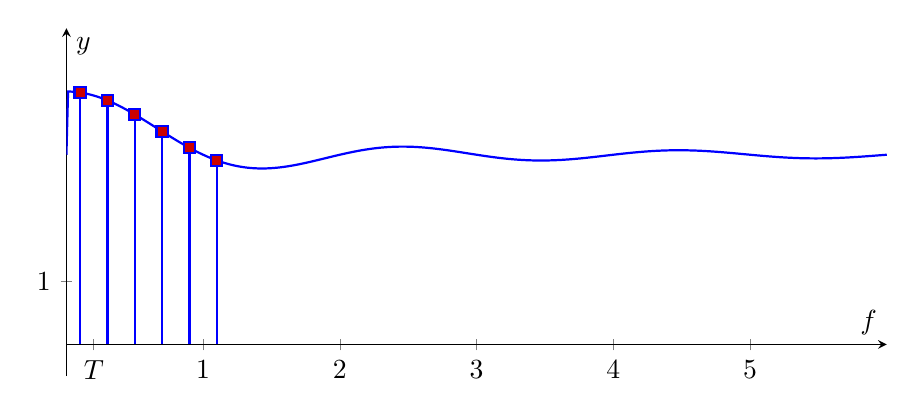
\begin{tikzpicture}
                        \begin{axis}[
                            domain=0:6,
                            samples=300,
                            axis lines=middle,
                            xlabel=$f$,
                            ylabel=$y$,
                            ymin=-0.5,
                            ymax=5,
                            xtick={0,0.2,1,2,3,4,5},
                            xticklabels={$0$,$T$,$1$,$2$,$3$,$4$,$5$},
                            ytick={1},
                            yticklabels={$1$},
                            width=12cm,
                            height=6cm
                        ]
                        \addplot [blue, thick,samples = 500] {(sin(deg(x*pi))/(x*pi))+3};
                        \addplot+ [ycomb,blue, thick, samples at = {0.1,0.3,0.5,0.7,0.9,1.1}] {(sin(deg(x*pi))/(x*pi))+3};
                        \end{axis}
                    \end{tikzpicture}
                    \caption{Campionamento MATLAB}
                    \label{fig:campionamento MATLAB xt}
                \end{figure}    
                \[
                    X_{(f)} \cong  T\sum_{n} x_{(nT)}e^{-j2\pi fnT}
                \]
                Ma nella $f$ è una variabile continua, quindi a sua volta bisogna variare $f$:\\
                \[X_{(fk)} =X_{(k\Delta f)} = \sum_{n} x_{(nT)}e^{-j2\pi \Delta fnT}T\]
                e la condizione sul $\Delta f$ è che $\Delta f<<BB$.
                \begin{figure}[H]
                    \centering
                    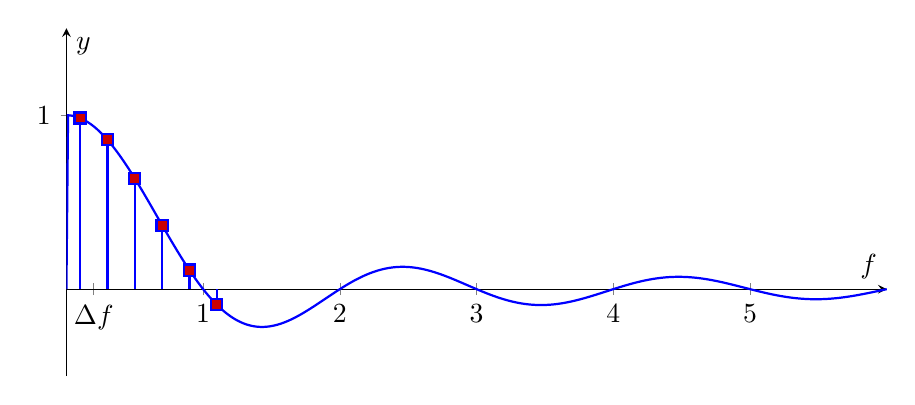
\begin{tikzpicture}
                        \begin{axis}[
                            domain=0:6,
                            samples=300,
                            axis lines=middle,
                            xlabel=$f$,
                            ylabel=$y$,
                            ymin=-0.5,
                            ymax=1.5,
                            xtick={0,0.2,1,2,3,4,5},
                            xticklabels={$0$,$\Delta f$,$1$,$2$,$3$,$4$,$5$},
                            ytick={1},
                            yticklabels={$1$},
                            width=12cm,
                            height=6cm
                        ]
                        \addplot [blue, thick,samples = 500] {sin(deg(x*pi))/(x*pi)};
                        \addplot+ [ycomb,blue, thick, samples at = {0.1,0.3,0.5,0.7,0.9,1.1}] {sin(deg(x*pi))/(x*pi)};
                        \end{axis}
                    \end{tikzpicture}
                    \caption{ $\Delta f$}
                    \label{fig:campionamento MATLAB sinc}
                \end{figure}
                Si può utilizzare anche la $FFT$ = Fast Fourier Transform
            }
            \item{
                Scala Logaritmica: $\eval*{x}_{db}= 10log_{10}(x)$
                \begin{table}[H]
                    \centering
                    \begin{tabular}{l|l}
                        x   & db  \\ 
                        \hline
                        2   & 3   \\
                        4   & 6   \\
                        8   & 9   \\
                        10  & 10  \\
                        1   & 0   \\
                        100 & 20  \\
                        200 & 23  \\
                        50  & 17 
                    \end{tabular}
                \end{table}
                Possiamo calcolare :
                \begin{itemize}
                    \item $\eval*{100}_{db} = 10log_{10}(100) =10log_{10}(10\dotproduct 10) = 10log_{10}(10)+10log_{10}(10) = 20db $
                    \item $\eval*{200}_{db} = 10log_{10}(100\dotproduct 2) = 10log_{10}(100)+10log_{10}(2) = 23db $
                    \item $\eval*{50}_{db} = 10log_{10}(10\dotproduct 5) = 10log_{10}(10)+10log_{10}(5) = 17db $
                \end{itemize}
            }
        \end{itemize}

        \begin{figure}[H]
            \centering
            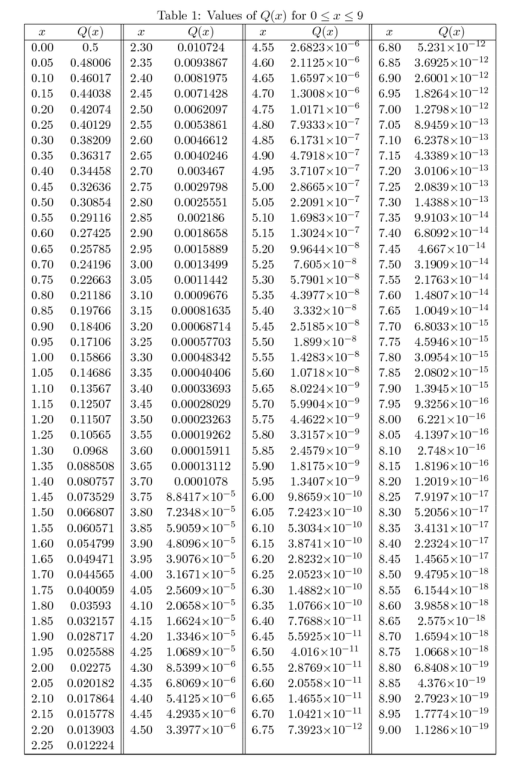
\includegraphics[width = \textwidth]{media/tabella funzione q.png}
        \end{figure}
